\chapter{Résultats}
%\addcontentsline{toc}{chapter}{Résultats}

\section{Étude de la pharmacocinétique du cetuximab chez l'Homme.}
\subsection{Introduction}
Comme nous l'avons vu plus haut (cf. 1.2.4 page 49) peu d'études ont analysé la pharmacocinétique du cetuximab chez l'Homme et aucune n'a analysé l'influence des insuffisances d'organes (insuffisance hépatique ou rénale) sur la pharmacocinétique des anticorps monoclonaux, même si on peut penser que la dialyse n'influence pas l'élimination des macromolécules comme les IgG. Une seule étude aborde la faisabilité d'utiliser du cetuximab et du bevacizumab chez un patient ayant un dysfonctionnement rénal, mais elle ne décrit pas la pharmacocinétique du cetuximab dans ce cas~\citep{REF135}.

L'utilisation du cetuximab en association à la radiothérapie est approuvée pour le traitement du cancer de la tête et du cou. La variabilité interindividuelle de la relation dose-concentration a été décrite par Dirks~\textit{et al.} dans cette pathologie~\citep{REF68}. Cependant, la pertinence des covariables identifiées dans cette étude doit être confirmée dans d'autres pathologies. Aucune étude n'a analysé la pharmacocinétique du cetuximab par approche compartimentale dans le cancer colorectal.
\subsection{Durant la dialyse rénale (publication~I)}
L'objectif de l'étude était d'étudier la pharmacocinétique du cetuximab chez un patient hémodialysé. Ce patient, âgé de 57~ans, mesurait 1,76~m pour 86~kg. Il était traité par cetuximab pour un carcinome épidermoïde infiltrant du sinus piriforme gauche T3N2bM0. Pour ce patient, la chirurgie et la chimiothérapie d'induction type TPF avaient été réfutées. Il recevait des doses de cetuximab de 250 mg/m$^2$ toutes les semaines et était hémodialysé trois fois par semaine, pendant cinq heures. Les concentrations sériques de cetuximab ont été mesurées au cours du temps par méthode ELISA (Publication~II) et la pharmacocinétique a été décrite par un modèle bi-compartimental avec constantes de distribution et d'élimination d'ordre~1 (Figure~\ref{fig:18}). Les volumes de distribution $V_1$ et $V_2$ ainsi que les clairances d'élimination et de distribution étaient respectivement estimés à 3,8~L ; 3,77~L ; 0,6 L$\cdot$jour$^{-1}$ et 0,53 L$\cdot$jour$^{-1}$. 
\begin{figure}[htbp]
	\centering
		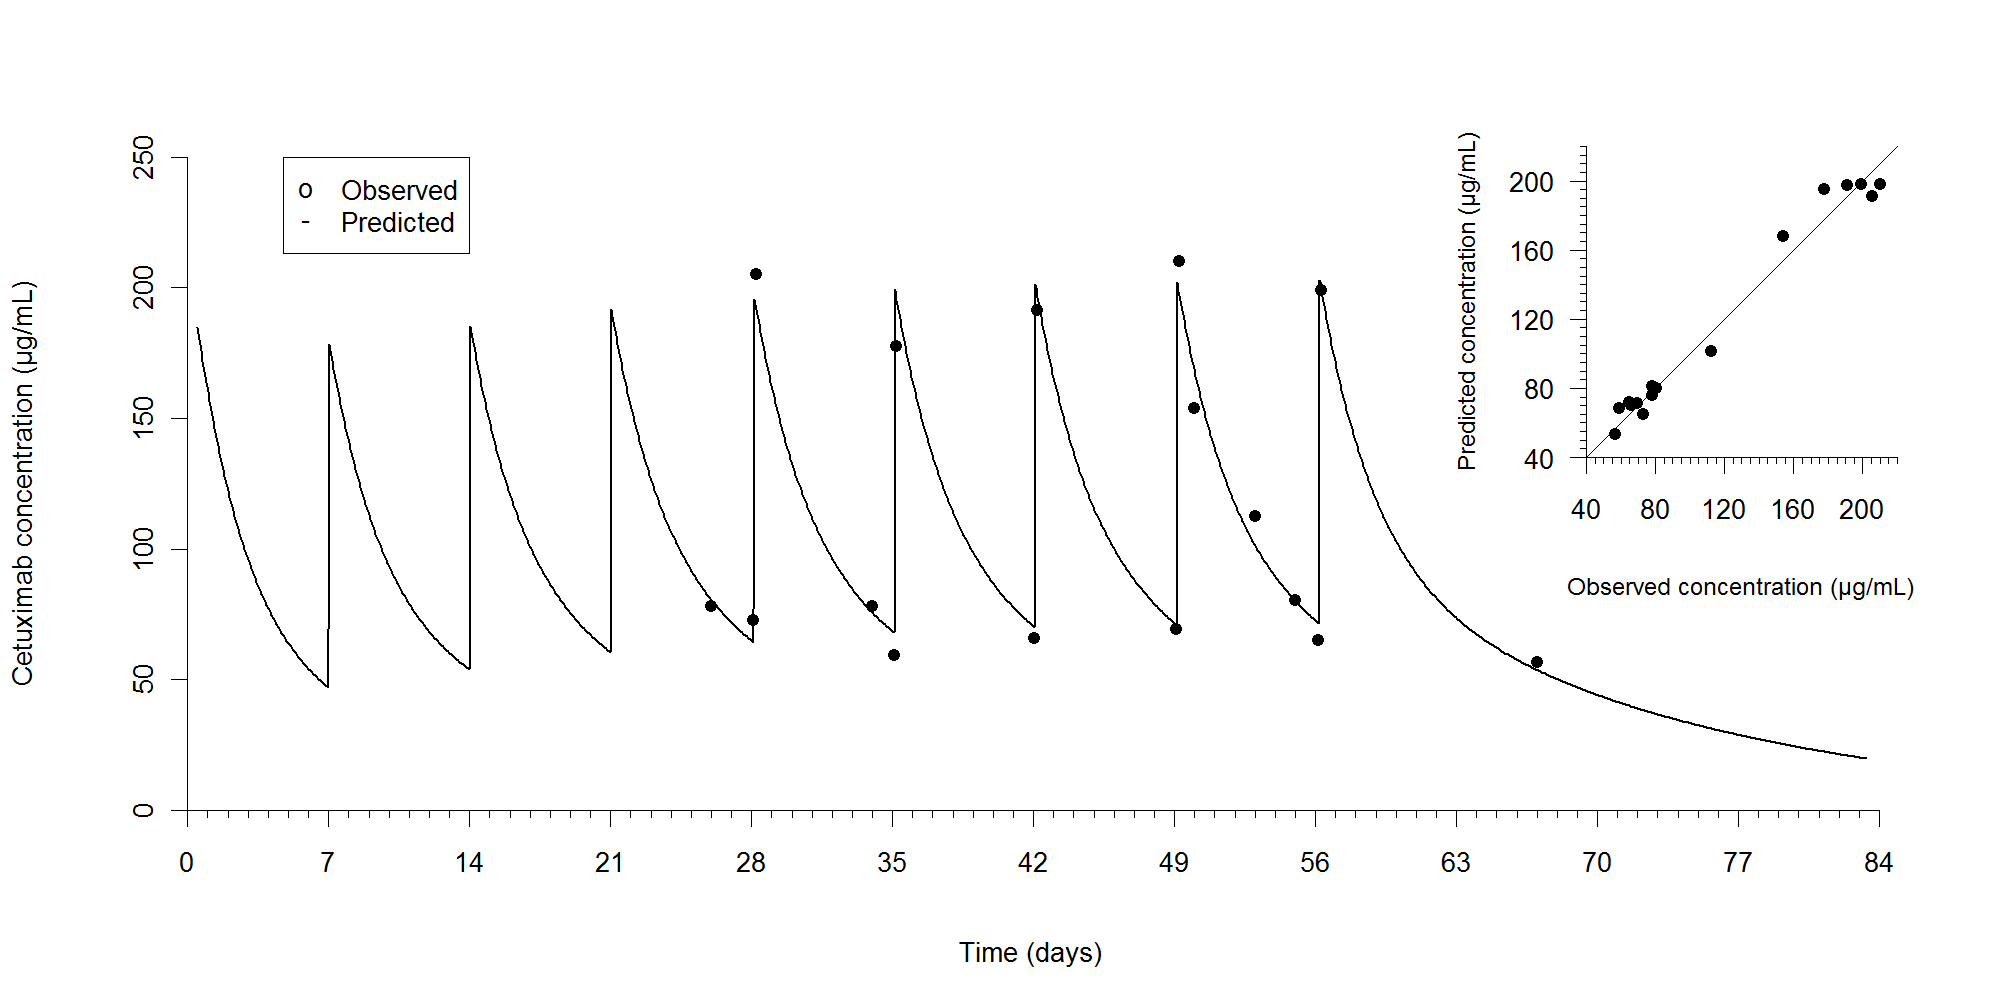
\includegraphics[width=10cm]{figures/raster/FIG_18}
	\caption[Concentration de cetuximab au cours du temps chez un patient hémodialysé.]{Concentration de cetuximab au cours du temps chez un patient hémodialysé. Les points sont les concentrations observées; la ligne, les concentrations prédites par un modèle à deux compartiments. Dans l'encadré, concentrations prédites vs concentrations observées.}
	\label{fig:18}
\end{figure}

Les estimations des paramètres ne permettaient pas de conclure à une influence du dysfonctionnement rénal ou de l'hémodialyse sur la pharmacocinétique du cetuximab chez ce patient. 
\subsection{Dans le cancer colorectal métastatique (publications~II et III)}
Dans la publication~II, les données de routine de 16 patients (15 traités pour cancer colorectal et 1 pour néoplasie indéterminée) ont été analysées par analyse pharmacocinétique de population. Le modèle décrivant le mieux les données était un modèle à 2 compartiments avec élimination d'ordre 1. Le faible nombre de prises de sang et de patients n'a pas permis d'appliquer un modèle plus complexe.

Le premier objectif de la publication~III était de décrire la pharmacocinétique du cetuximab chez des patients atteints de cancer colorectal métastatique et d'en identifier les sources de variabilité. 

Il s'agissait d'une étude ancillaire d'un essai de phase~II multicentrique (FOLFIRICETUX) qui a évalué la tolérance d'un schéma FOLFIRI (acide folinique, 5-fluorouracile [5-FU] et irinotécan), optimisé en prenant en compte de la pharmacogénomique de l'irinotecan et de la pharmacocinétique du 5-FU et associé au cetuximab administré de façon hebdomadaire. La dose d'irinotecan était adaptée individuellement en fonction du polymorphisme génétique de la partie promotrice d'UGT1A1. Les patients 6/7 avaient une dose inchangée de 180~mg/m$^2$. Les patients 7/7 avaient une dose initiale réduite de 30\% (126~mg/m$^2$). Les patients ayant un autre polymorphisme UGT1A1 avaient une dose initiale de 180~mg/m$^2$ augmentée à chaque cycle de 20\% si la tolérance le permettait jusqu'à une dose maximale de 300~mg/m$^2$. Les doses de 5-FU étaient adaptées au statut de la dihydropyrimidine déshydrogénase (DPD) et à chaque cycle, à la pharmacocinétique du 5-FU.

Entre 2007 et 2009, 96 patients ont été inclus (homme 58 \%, âge moyen : 63 ans [38-80]). Il s'agissait d'un traitement de 2ème ligne chez 82\% des patients. Le cetuximab était administré de façon conventionnelle : une dose de charge de 400~mg/m$^2$ suivie d'injections de 250~mg/m$^2$ toute les semaines. 

Un total de 1322 concentrations sériques de cetuximab a été mesuré avec un nombre moyen de 13 concentrations par patient. Les concentrations sériques résiduelles de cetuximab variaient entre la limite inférieure de quantification (0,75~mg/L) et 300~mg/L.

La pharmacocinétique du cetuximab a été décrite au moyen d'un modèle à 2~compartiments combinant une élimination d'ordre~1 et une élimination d'ordre~0 (Figure~\ref{fig:19}D). Le modèle d'erreur était proportionnel et les 13~concentrations inférieures à la LLOQ ont été censurées. Ce modèle a permis une description satisfaisante des concentrations et notamment des résiduelles très basses (graphiques diagnostiques Figures~\ref{fig:20}-\ref{fig:22}). Le remplacement de l'élimination d'ordre~0 par une élimination de type Michaelis-Menten ne diminuait pas significativement la valeur de la fonction objective. De plus, la valeur de $k_M$ obtenue était inférieure à la LLOQ et n'était donc pas pertinente. Les valeurs de population des cinq paramètres du modèle final étaient correctement estimées avec un CV inférieur à 10\%. Ces valeurs sont présentées dans le Tableau~\textbf{3}. La surface corporelle est apparue comme étant une covariable significative de $V_1$, $V_2$ et $k_0$, ces paramètres augmentant avec sa valeur. L'albuminémie initiale était une covariable significative de $\CL$ : la clairance était d'autant plus importante que l'albuminémie était faible.


\begin{figure}[htbp] 

  \begin{subfigure}[b]{0.75\linewidth}
    \centering
    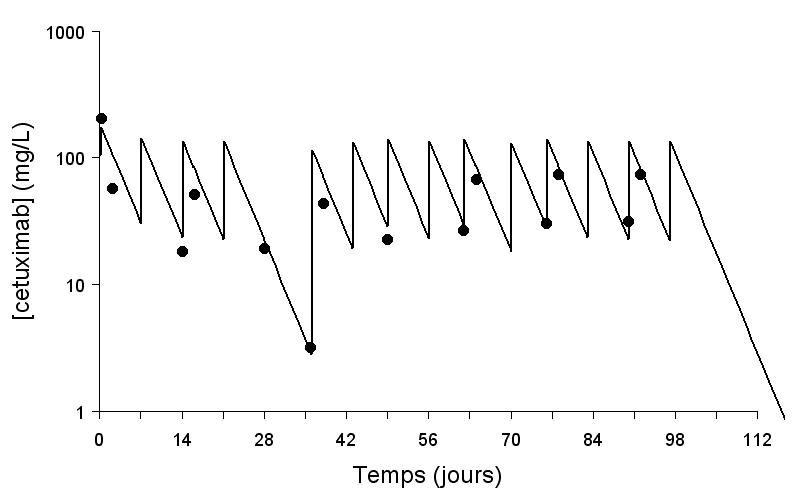
\includegraphics[width=0.75\linewidth]{figures/raster/FIG_19a1} 
  \end{subfigure}%% 
  \begin{subfigure}[b]{0.25\linewidth}
    \centering
    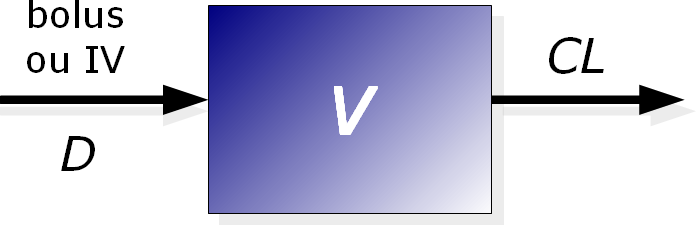
\includegraphics[width=0.75\linewidth]{figures/raster/FIG_19a2} 
  \end{subfigure} 
  
  \begin{subfigure}[b]{0.75\linewidth}
    \centering
    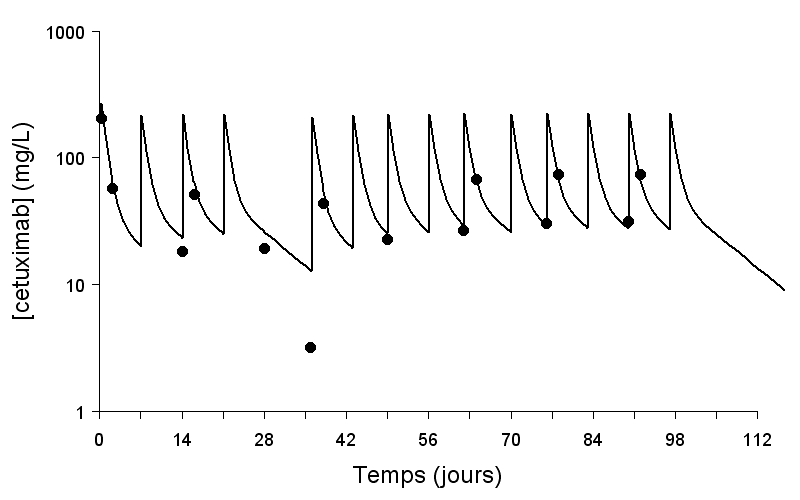
\includegraphics[width=0.75\linewidth]{figures/raster/FIG_19b1} 
  \end{subfigure}%%
  \begin{subfigure}[b]{0.25\linewidth}
    \centering
    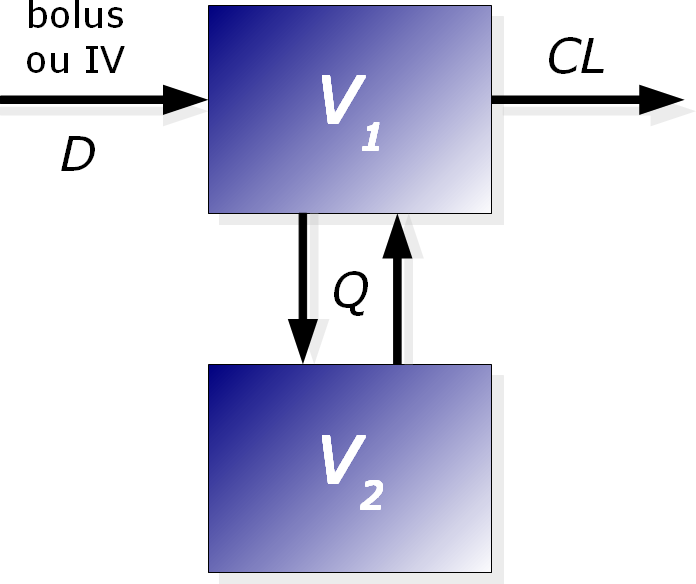
\includegraphics[width=0.75\linewidth]{figures/raster/FIG_19b2} 
  \end{subfigure} 
  
  
  \begin{subfigure}[b]{0.75\linewidth}
    \centering
    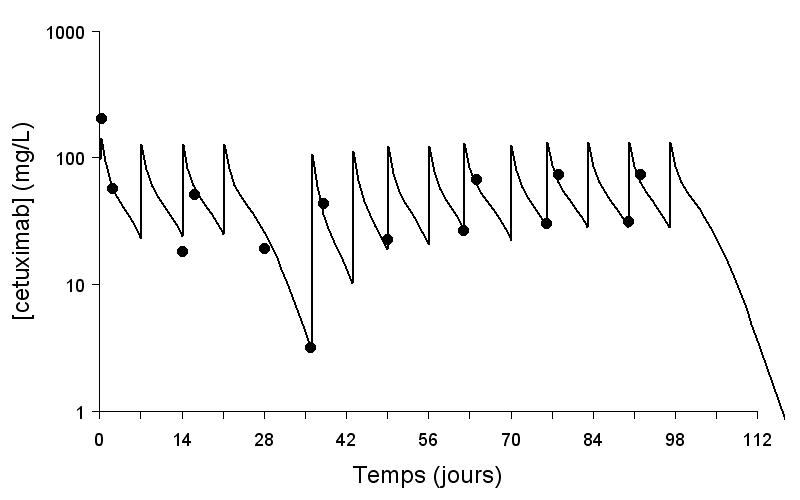
\includegraphics[width=0.75\linewidth]{figures/raster/FIG_19c1} 
  \end{subfigure}%%
  \begin{subfigure}[b]{0.25\linewidth}
    \centering
    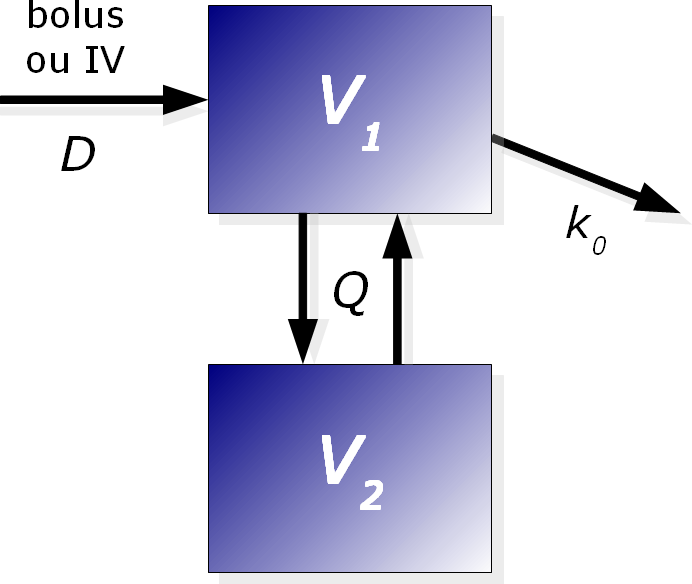
\includegraphics[width=0.75\linewidth]{figures/raster/FIG_19c2} 
  \end{subfigure} 
  
  
  \begin{subfigure}[b]{0.75\linewidth}
    \centering
    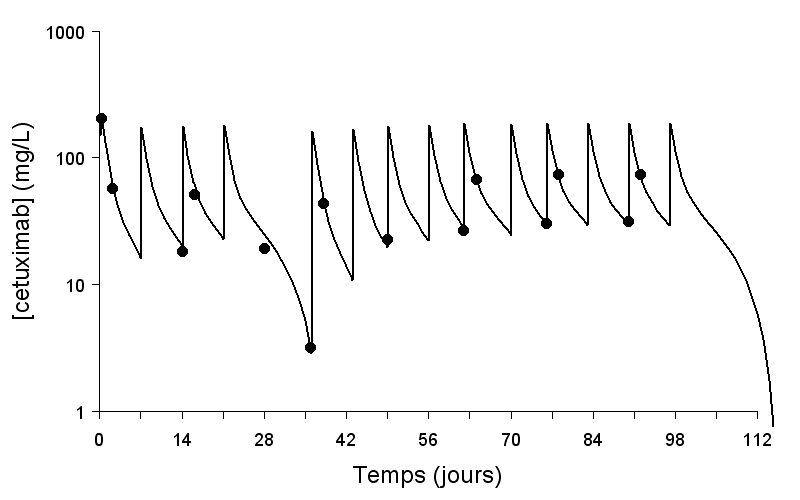
\includegraphics[width=0.75\linewidth]{figures/raster/FIG_19d1} 
  \end{subfigure}%%
  \begin{subfigure}[b]{0.25\linewidth}
    \centering
    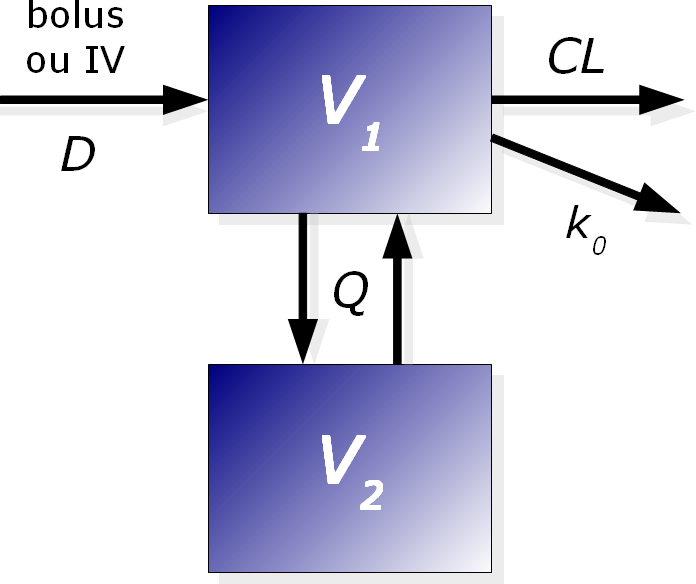
\includegraphics[width=0.75\linewidth]{figures/raster/FIG_19d2} 
  \end{subfigure} 
  
  \caption[Profils PK d'un patient avec les différents modèles]{Exemples de profils pharmacocinétiques d'un patient obtenus avec les différents modèles testés. \textbf{A} et \textbf{B} : modèles à un et deux compartiments avec élimination d'ordre~1 ($\CL$). \textbf{C} : modèle à deux compartiments avec élimination d'ordre 0 ($k_0$). La meilleure description des concentrations observées est obtenue avec le dernier modèle (\textbf{D}) combinant une élimination d'ordre~0 et une élimination d'ordre~1.}
  \label{fig:19} 
\end{figure}

\begin{table}[!ht]
  \centering
  \caption{Valeur estimées des paramètres pharmacocinétique du cetuximab dans l'étude de la publication III.}
    \begin{tabular}{lcccl}
       &  &  &  &  \\
      \hline
      \textbf{} & \textbf{paramètre} & \textbf{s.e.} & \textbf{r.s.e.(\%)} & $p$ \\
      \hline
      \hline
      $V_1$ (L) & 2,96 & 0,12 & 4 &  \\
      $\CL$ (L/jour) & 0,497 & 0,021 & 4 &  \\
      $V_2$ (L) & 4,65 & 0,29 & 6 &  \\
      $Q$ (L/day) & 0,836 & 0,07 & 8 &  \\
      $k_0$ (mg/jour) & 8,71 & 0,84 & 10 &  \\
       &  &  &  &  \\
      $\beta_{V_1,BSA}$ & 0,42 & 0,17 & 41 & 0,015 \\
      $\beta_{V_2,BSA}$ & 0,56 & 0,27 & 49 & 0,039 \\
      $\beta_{k_0,BSA}$ & 1,58 & 0,35 & 22 & 0,0000078 \\
      $\beta_{\CL,Alb}$  & -0,0244 & 0,009 & 37 & 0,0064 \\
       &  &  &  &  \\
      $\omega^2_{V_1}$ & 0,0725 & 0,02 & 28 &  \\
      $\omega^2_{\CL}$ & 0,11 & 0,018 & 17 &  \\
      $\omega^2_{V_2}$ & 0,21 & 0,048 & 23 &  \\
      $\omega^2_{Q}$ & 0,305 & 0,076 & 25 &  \\
      $\omega^2_{k_0}$ & 0,215 & 0,041 & 19 &  \\
       &  &  &  &  \\
      $\sigma^2_{prop}$ & 0,222 & 0,0053 & 2 &  \\
      \hline
    \end{tabular}
  \label{tab:3}
\end{table}
 
\begin{figure}[htbp]
	\centering
		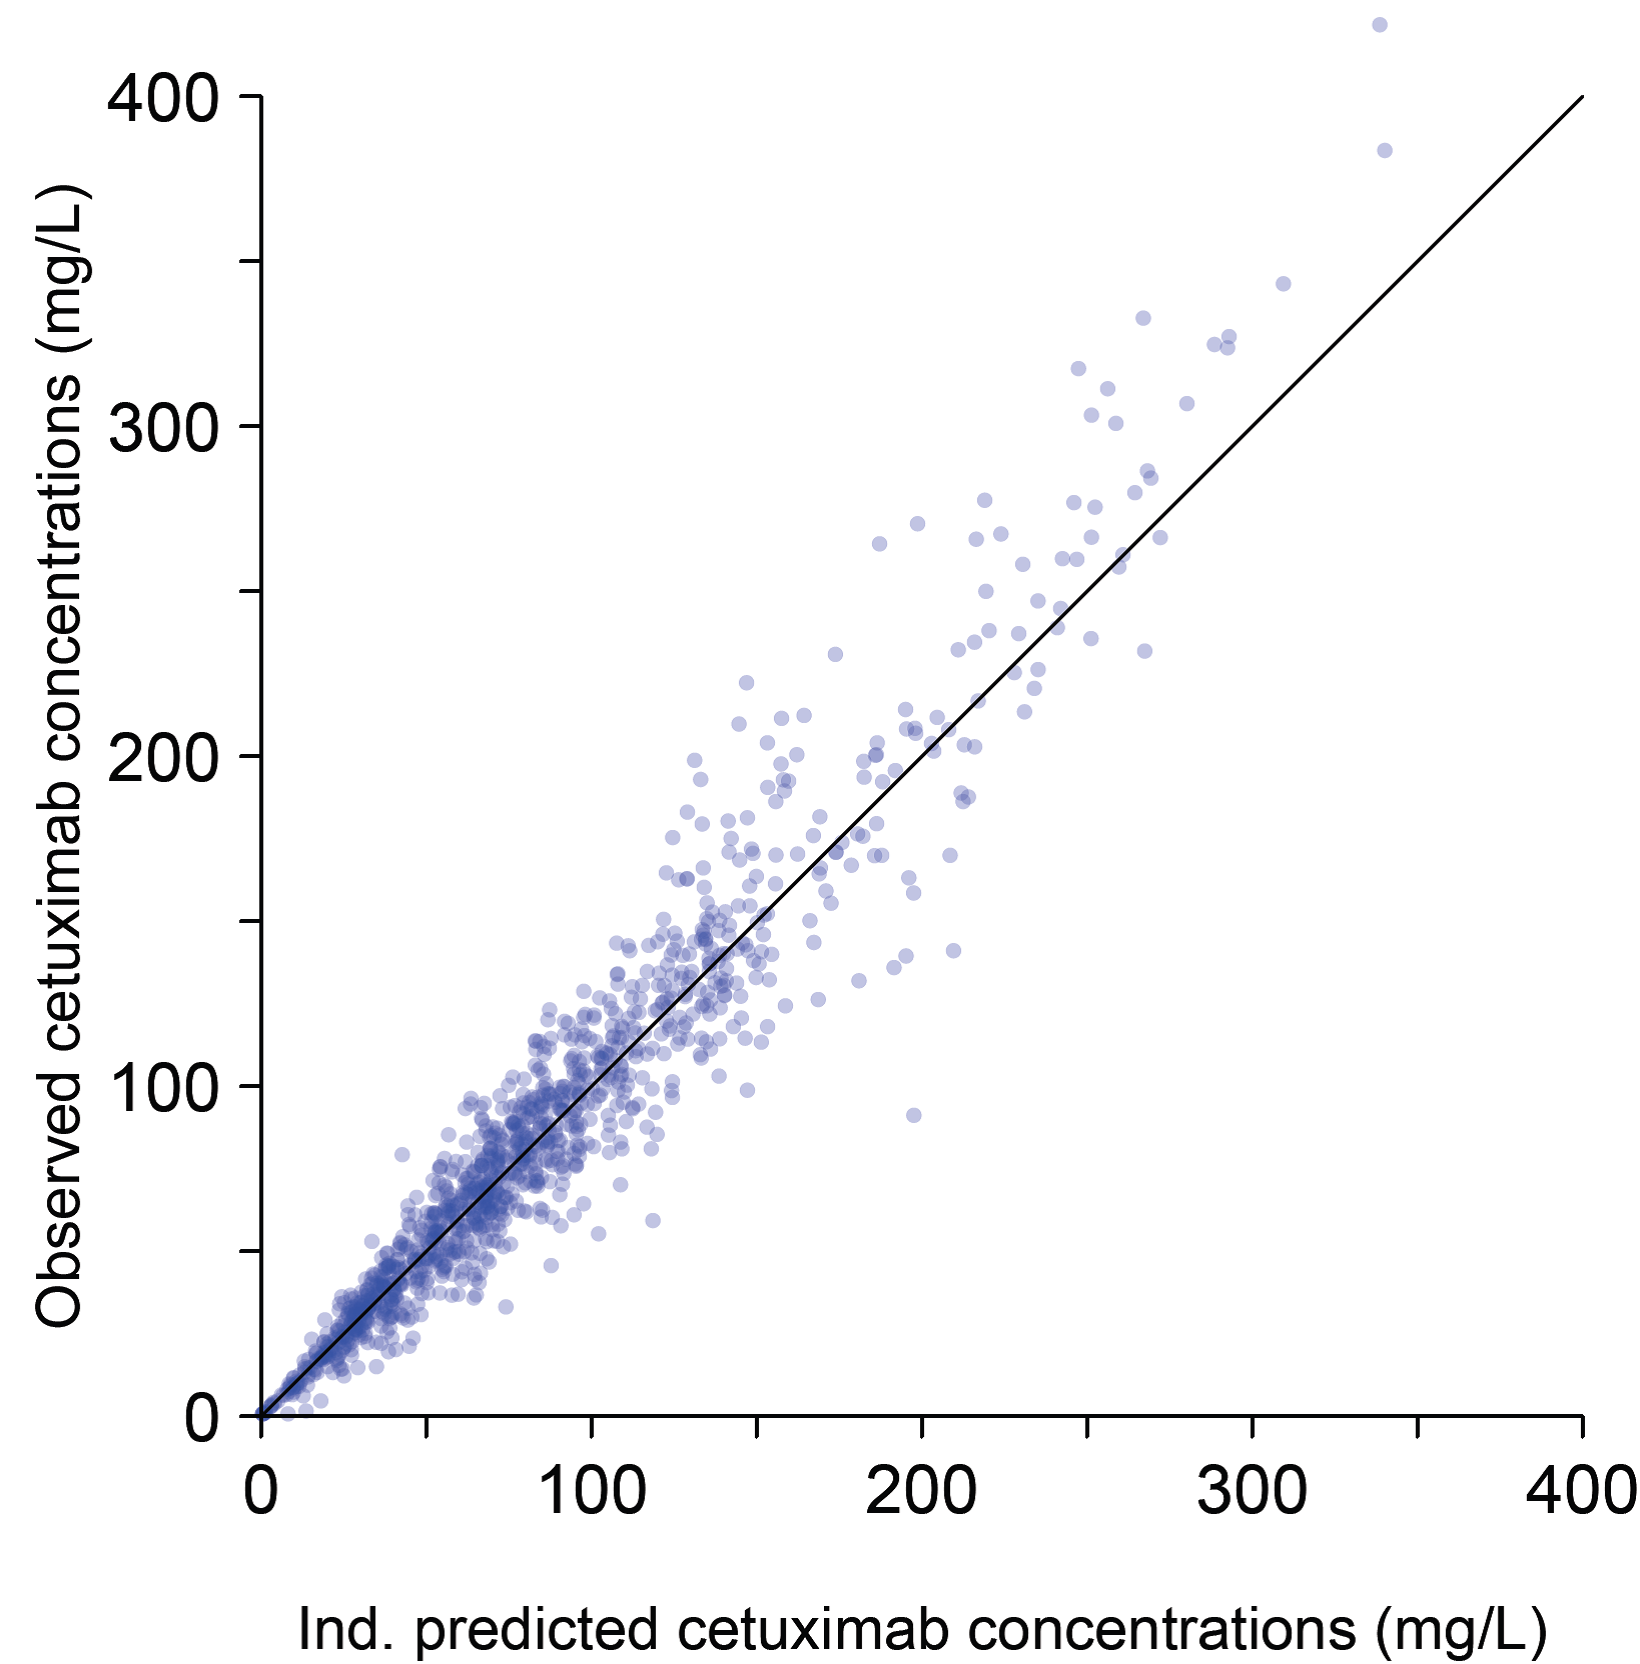
\includegraphics[width=10cm]{figures/raster/FIG_20}
	\caption{Concentrations de cetuximab observées chez des patients traités pour cancer colorectal métastatique vs. concentrations prédites au moyen d'un modèle à 2 compartiments combinant une élimination d'ordre~1 et une élimination d'ordre~0.}
	\label{fig:20}
\end{figure}

\begin{figure}[htbp]
	\centering
		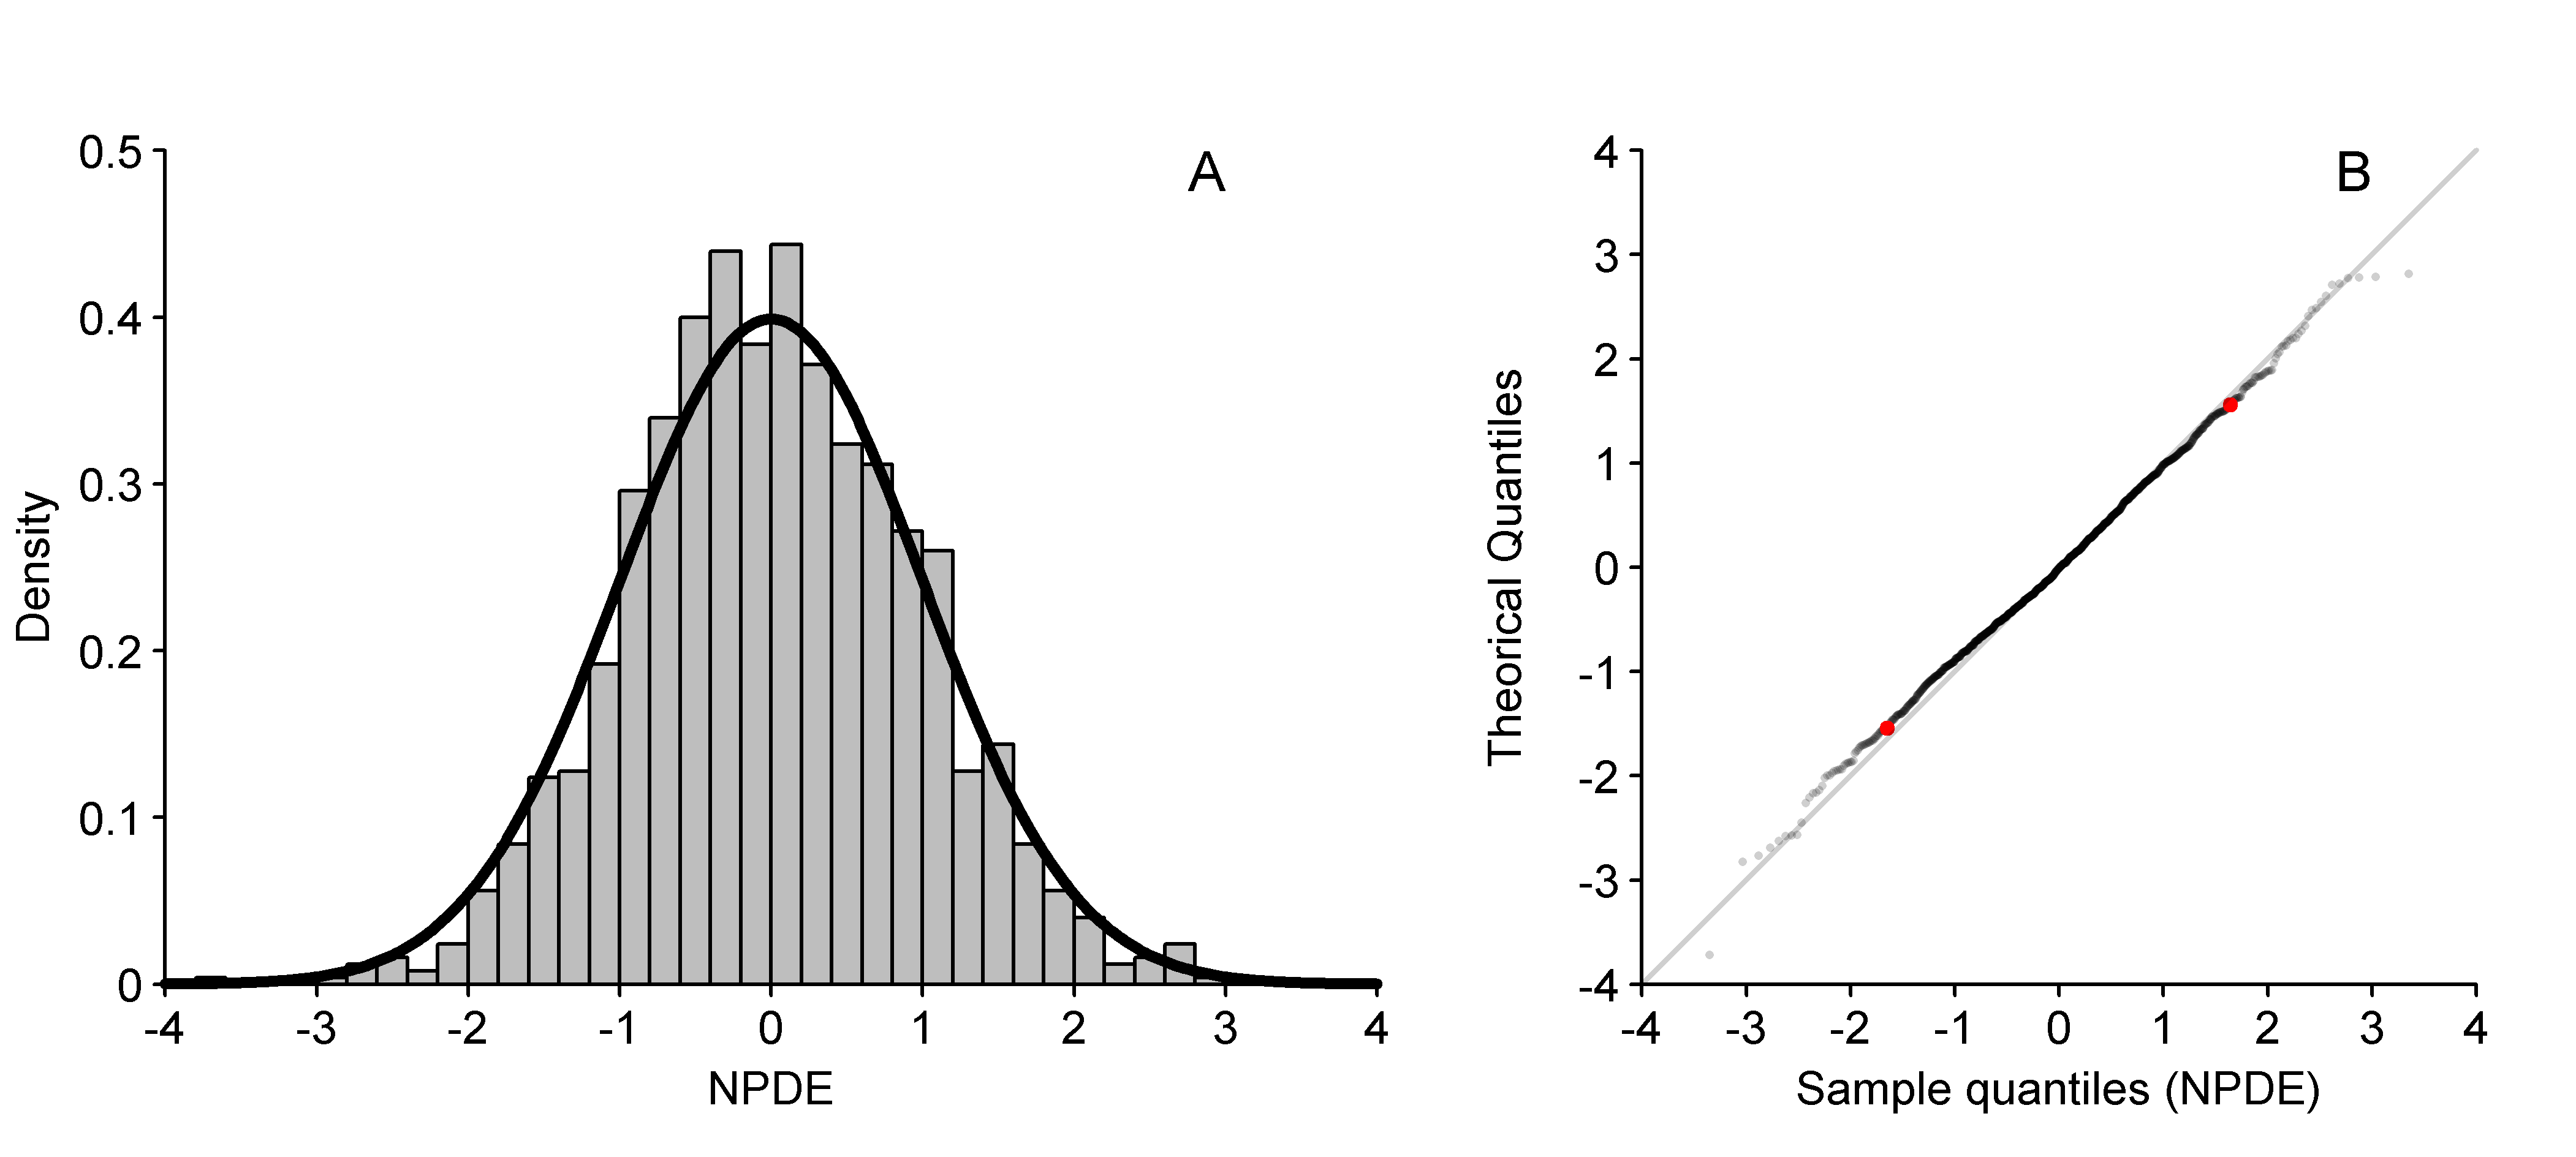
\includegraphics[width=10cm]{figures/raster/FIG_21}
	\caption{Distribution normalisée des résidus (Normalized prediction distribution errors, NPDE). (A) : distribution (histogramme) et densité de probabilité de la loi normale centrée réduite (courbe). (B) : quantiles des NPDE \textit{vs.} quantiles de la loi normale centrée réduite. En rouge, les 5éme et 95éme percentiles.}
	\label{fig:21}
\end{figure}
\begin{figure}[htbp]
	\centering
		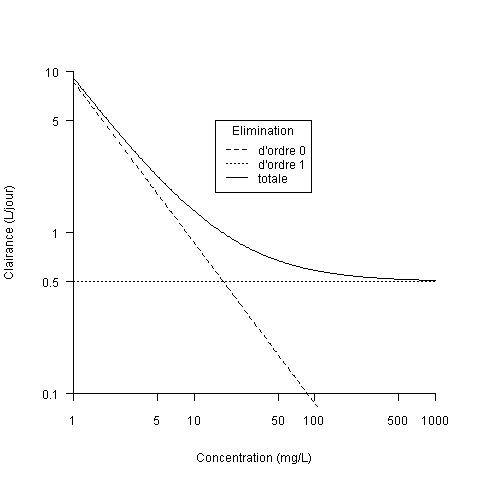
\includegraphics[width=10cm]{figures/raster/FIG_22}
	\caption{Clairance d'élimination en fonction de la concentration de cetuximab. L'élimination globale du cetuximab (en noir) a été décrite comme la combinaison d'une élimination d'ordre~1 (pointillés) et d'une élimination d'ordre 0 (tirets).}
	\label{fig:22}
\end{figure}

\subsection{Conclusion sur la pharmacocinétique du cetuximab chez l'Homme.}
Les études des publications~II et III ont permis d'obtenir les premières descriptions compartimentales de la pharmacocinétique du cetuximab chez l'Homme dans le cas d'un dysfonctionnement rénal et dans le cas du cancer colorectal métastatique. Le modèle de l'étude~IV était identifiable "grâce" aux pauses thérapeutiques qui ont eu pour conséquence des concentrations résiduelles très basses.

Le modèle utilisé dans l'étude~IV (FOLFIRICETUX) n'est pas significativement meilleur pour décrire les concentrations du patient de l'étude~III (patient hémodialysé) que le modèle à deux compartiments avec élimination d'ordre~1. Dans l'étude~IV, des modèles plus complexes (Michaelis-Menten, TMDD...) ont été testés mais n'étaient pas applicables en raison du nombre insuffisant de données. 

\section{Influence de la pharmacocinétique du cetuximab sur son efficacité (publication~III)}
\subsection{Modélisation pharmacocinétique-pharmacodynamique}
Les connaissances de la relation concentration-effet du cetuximab sont assez limitées 122. Les études concernant l'influence du polymorphisme \textit{FCGR3A}-V158F portent sur la relation dose-effet alors que ce facteur génétique devrait concerner la relation concentration-effet du cetuximab.

La recherche d'un modèle PK-PD stable avec prise en compte ou non des doses de la chimiothérapie associée a été réalisée. Les critères d'efficacité étudiés étaient le critère RECIST, l'ACE et le CA 19.9 ainsi que leurs valeurs relatives par rapport à celles mesurées à l'initiation du traitement. Les modèles TMDD ou PK-PD indirects n'ont pas permis pas de décrire les données pharmacodynamiques, car les paramètres de ces modèles n'étaient pas identifiables. Puisque les données disponibles apparaissaient insuffisantes pour décrire la relation concentration-effet, nous avons choisi de décrire la relation entre concentration et survie sans progression, par approche paramétrique, puis semi-paramétrique.

Dans la cohorte de la publication III, la médiane de survie sans progression (PFS) était de 6,5 mois pour l'ensemble des 96~patients inclus (Figure~\ref{fig:23}). 
\begin{figure}[htbp]
	\centering
		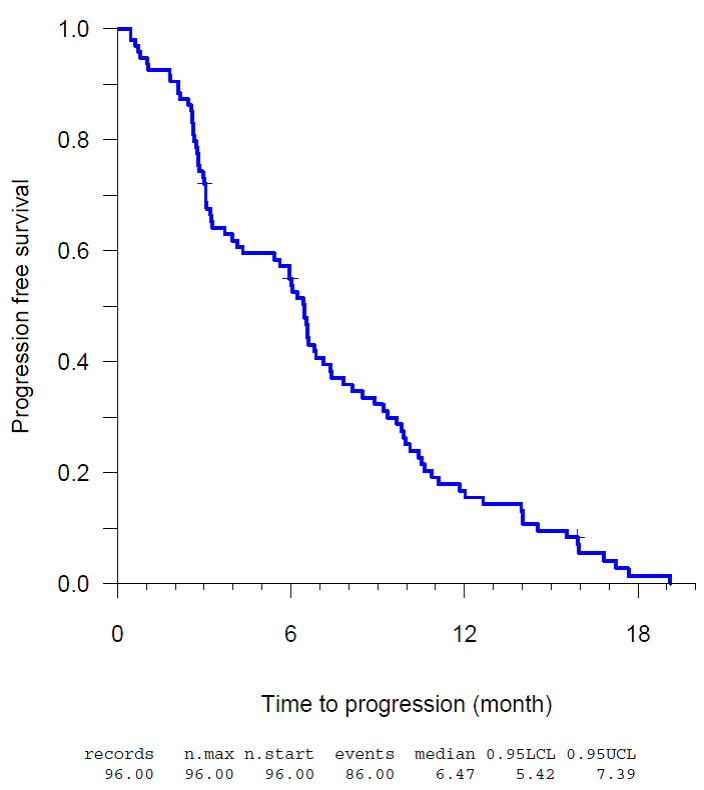
\includegraphics[width=6cm]{figures/raster/FIG_23}
	\caption[PFS de 96 patients]{Survie sans progression (PFS) des 96 patients traités par cetuximab pour cancer colorectal métastatique.}
	\label{fig:23}
\end{figure}
L'influence sur la PFS des facteurs suivant a été recherchée :
\begin{itemize}
\item exposition au cetuximab et paramètres pharmacocinétiques du cetuximab,
\item facteurs génétiques reliés au cetuximab (statut \textit{KRAS} tumoral et polymorphisme \textit{FCGR3A}-V158F),
\item dose moyenne et nombre d'injections de la chimiothérapie associée,
\item et polymorphismes reliés à cette chimiothérapie.
\end{itemize}
L'approche de modélisation de la PFS utilisée a d'abord été paramétrique, par modèle de Weibull. Le modèle ne permettait cependant pas de décrire de façon satisfaisante les fonctions de survie de sous-groupes de patients. Pour cette raison, nous avons utilisé un modèle de Cox.
\subsection{Influence de l'exposition au cetuximab sur la PFS}
L'$\AUC$ est le meilleur reflet de l'exposition. Cependant, c'est une valeur qui varie au cours du temps : un patient qui a progressé au bout de 6 mois a, à ce moment-là, une $\AUC$ approximativement deux fois supérieure à celle d'un patient qui a progressé (et donc arrêté son traitement) trois mois plus tôt. Un tel paramètre dit "temps-dépendant" peut être intégré dans un modèle de Cox mais son interprétation est difficile. Afin d'obtenir un facteur indépendant du temps, nous avons normalisé l'$\AUC$ par la dose cumulée. Cette $\AUC$ normalisée ($\AUC_n$) avait la dimension d'un temps par unité de volume ([T]$\cdot$[L]$^{-3}$). Pour faciliter l'interprétation, la "clairance globale" qui correspond à l'inverse de l'$\AUC_n$ a été préférée (Volume par unité de temps). La clairance globale a été calculée par l'équation~\ref{eq:11}, l'$\AUC$ étant estimée par approche compartimentale.

Les patients dont la clairance globale était inférieure à la valeur médiane (0,66~L/jour) avaient un temps de progression médian plus long que ceux dont la clairance globale était supérieure à la valeur médiane (8,9 mois vs 3,3 mois) et un risque relatif de progression 2,6 fois moins élevé (p < 5 $\cdot$ 10$^{-5}$) (Figure~\ref{fig:24}). 
\begin{figure}[htbp]
	\centering
		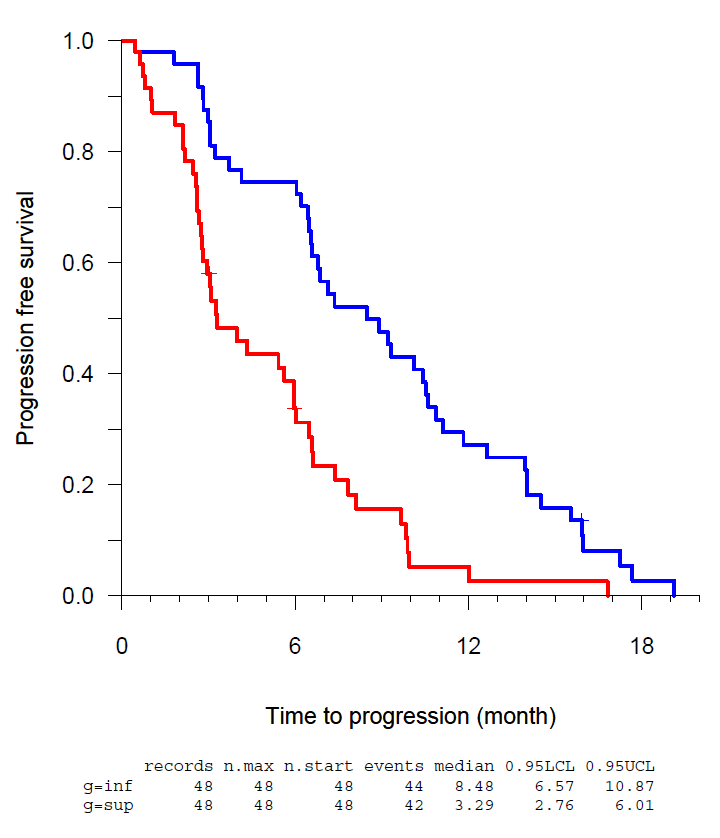
\includegraphics[width=6cm]{figures/raster/FIG_24}
	\caption{Survie sans progression (PFS) selon la clairance globale médiane (0,66 L/jour). En bleu, le groupe des patients ayant une clairance globale inférieure à la médiane ($n = 48$) ; en rouge le groupe des patients ayant une clairance globale supérieure à la médiane ($n = 48$) ($p < 0,00005$).}
	\label{fig:24}
\end{figure}
Le statut \textit{KRAS} de la tumeur des patients inclus dans l'étude a pu être déterminé rétrospectivement chez 51 patients et la tumeur était non mutée \textit{KRAS} chez 32 d'entre eux. Dans cette étude, la PFS n'était pas influencée par le statut \textit{KRAS} tumoral ($p = 0,66$) (Figure~\ref{fig:25}).
\begin{figure}[htbp]
	\centering
		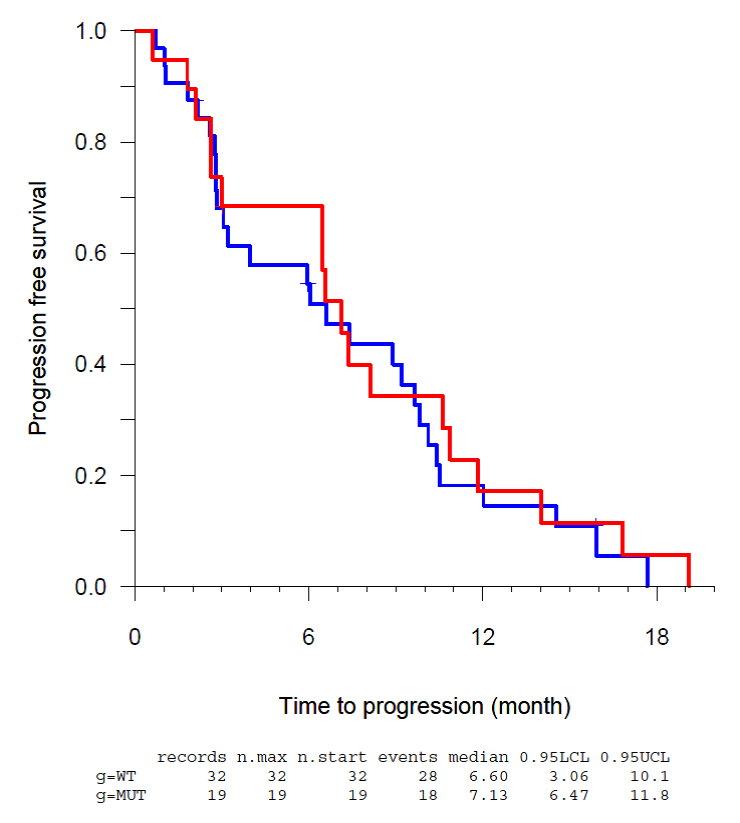
\includegraphics[width=6cm]{figures/raster/FIG_25}
	\caption{Survie sans progression (PFS) selon le statut \textit{KRAS} tumoral. En bleu, le groupe des patients portant une tumeur non mutés \textit{KRAS} ; en rouge le groupe des patients porteur de tumeur mutée \textit{KRAS} ($p = 0,66$).}
	\label{fig:25}
\end{figure}
Parmi les patients avec une tumeur non mutée \textit{KRAS}, ceux dont la clairance globale était inférieure à la valeur médiane avaient un temps de progression médian plus long que les autres (10,1 mois \textit{vs.} 2,8 mois). Ces patients avaient également un risque de progression 2,8 fois moins élevé ($p = 0,014$). Cette différence n'était pas significative chez les patients ayant une tumeur mutée \textit{KRAS} ($p = 0,21$) (Figure~\ref{fig:26}).
\begin{figure}[htbp]
	\centering
		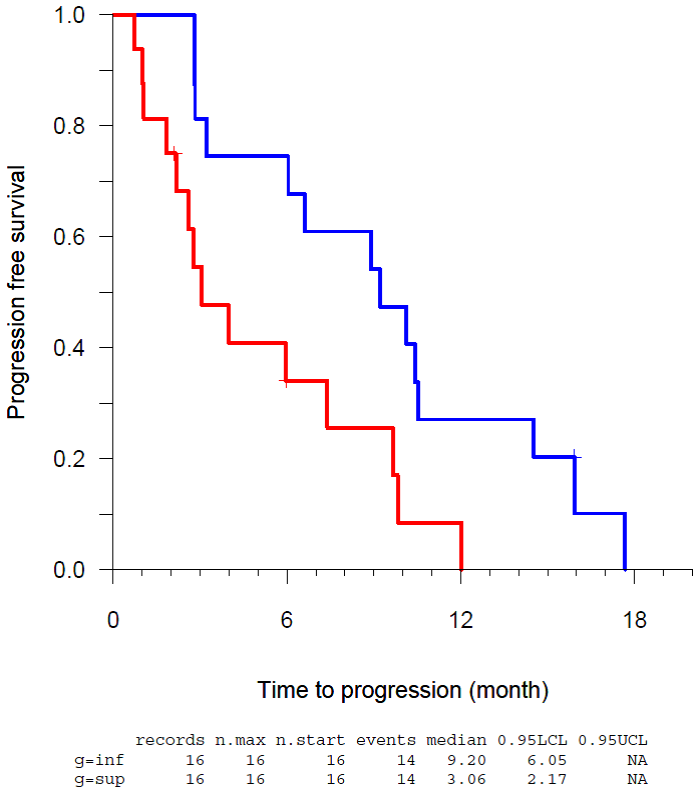
\includegraphics[width=6cm]{figures/raster/FIG_26a}
		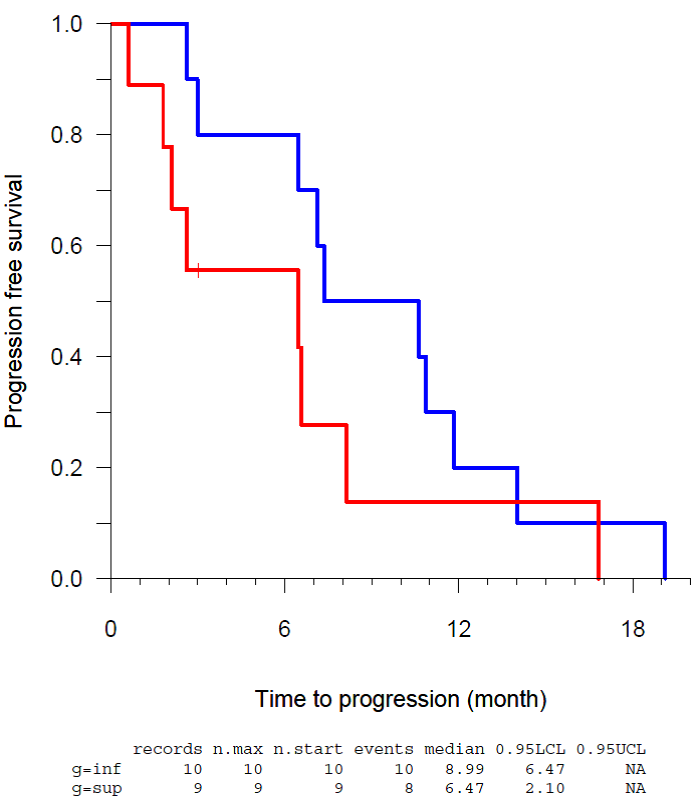
\includegraphics[width=6cm]{figures/raster/FIG_26b}
	\caption{Survie sans progression (PFS) selon la clairance globale médiane. A gauche, le groupe des patients portant une tumeur non mutés \textit{KRAS} ($p = 0,014$); A droite, le groupe des patients porteur de tumeur mutée \textit{KRAS} ($p = 0,21$) - En bleu, le groupe des patients ayant une clairance globale inférieure ou égale à la médiane ; en rouge le groupe des patients ayant une clairance globale supérieure à la médiane.}
	\label{fig:26}
\end{figure} 
Dans cette étude, le polymorphisme \textit{FCGR3A}-V158F n'influençait pas significativement la PFS. Dans le sous-groupe des patients \textit{KRAS} non mutés, six patients étaient homozygotes \textit{FCGR3A}-V/V. Cependant, parmi ces six patients, trois n'ont plus reçu de cetuximab après 6 mois de traitement, ce qui pourrait expliquer la perte de l'avantage d'être \textit{FCGR3A}-V/V (Figure~\ref{fig:27}). 
\begin{figure}[htbp]
	\centering
		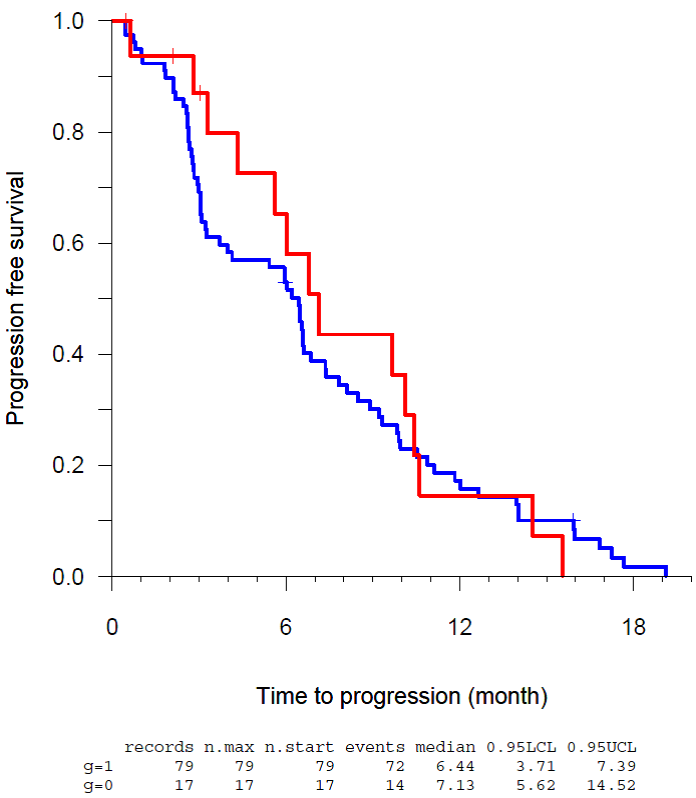
\includegraphics[width=6cm]{figures/raster/FIG_27a}
		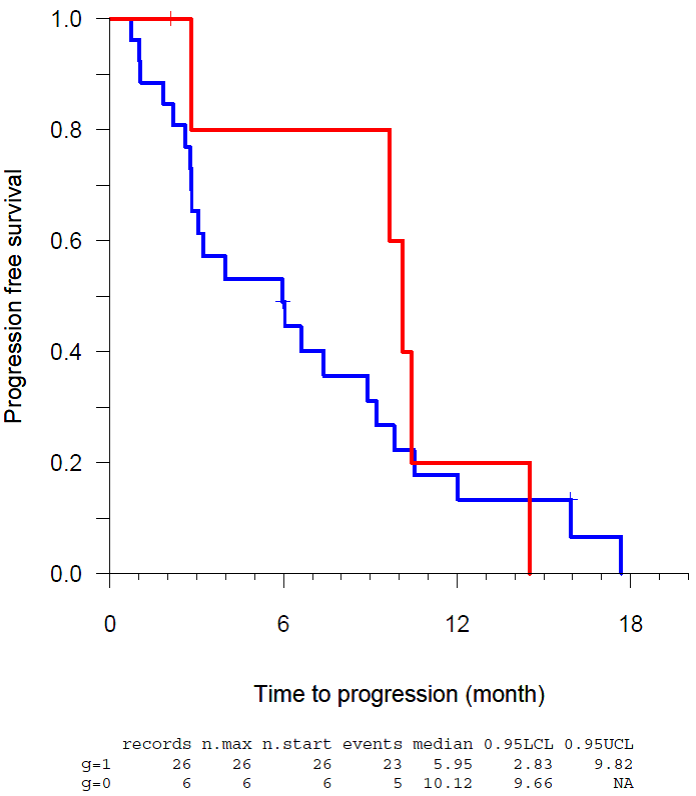
\includegraphics[width=6cm]{figures/raster/FIG_27b}
		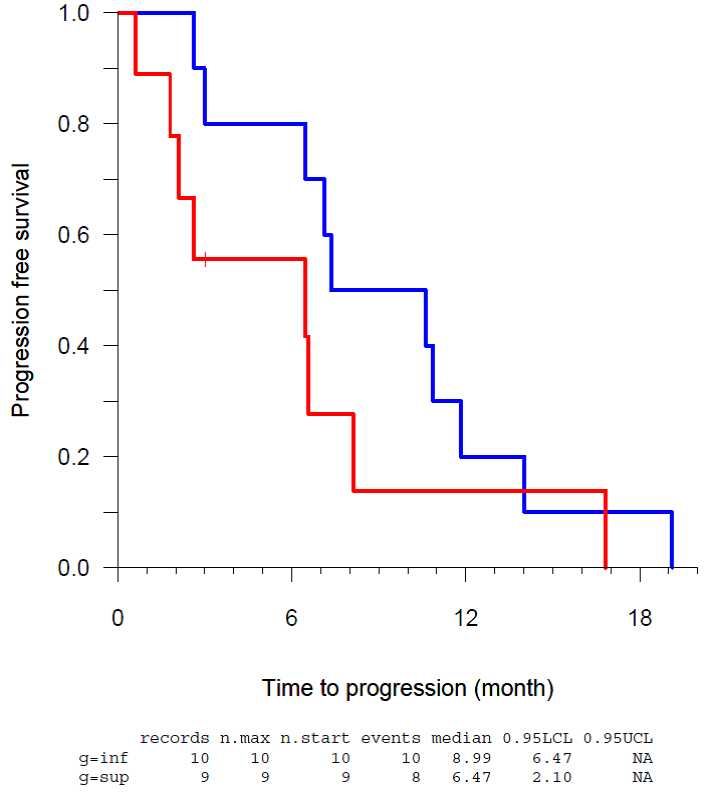
\includegraphics[width=6cm]{figures/raster/FIG_27c}
	\caption{Survie sans progression (PFS) selon le polymorphisme \textit{FCGR3A}-V158F. A gauche, chez les 96 patients ; au milieu, chez les patients porteurs de tumeur non mutée \textit{KRAS} ; à droite, chez les patients porteur de tumeur mutée \textit{KRAS} - En rouge, patients homozygotes \textit{FCGR3A}-V/V ; en bleu, patients porteurs de l'allèle \textit{FCGR3A}-F.}
	\label{fig:27}
\end{figure}
\subsection{Relation entre la toxicité et la PFS}
Nous avons étudié la relation entre la PFS et la présence/absence de toxicité cutanée et une toxicité cutanée supérieure ou non au grade~1, à J7, J14 et J21. La relation entre la PFS et la toxicité cutanée à 21 jours n'était pas significative ($p = 0,077$, Figure~\ref{fig:28}).
Cependant, $k_0$ était significativement plus important chez les patients ayant présenté une toxicité cutanée pendant les 21 premiers jours de traitement ($p = 0,04$). De plus, les valeurs de $k_0$ étaient significativement plus élevées chez les patients ayant présenté un grade de toxicité cutanée supérieur à 1 avant J7 et J14 (respectivement $p = 0,014$ et $p = 0,04$).
\begin{figure}[htbp]
	\centering
		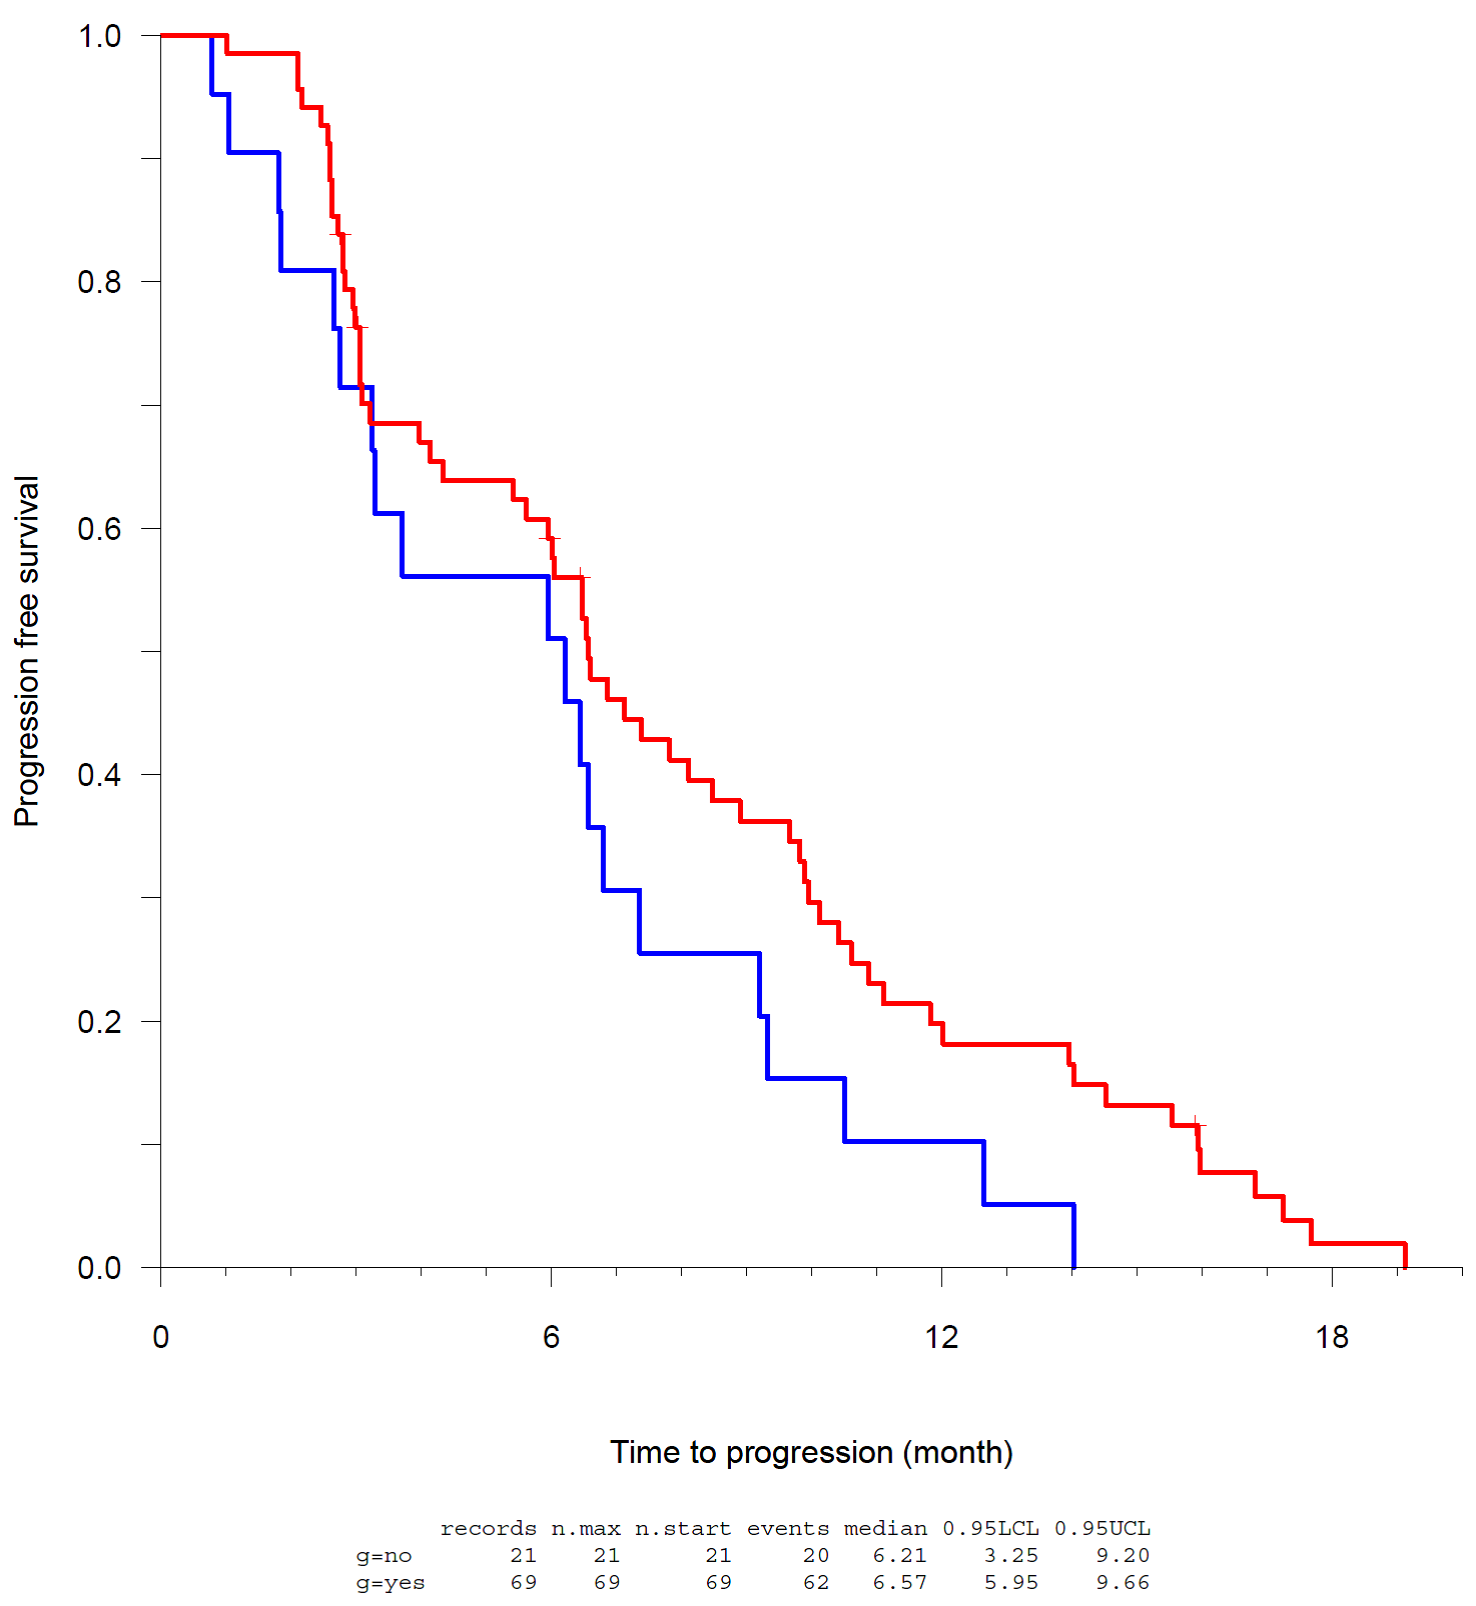
\includegraphics[width=6cm]{figures/raster/FIG_28}
	\caption{Survie sans progression (PFS) selon la toxicité cutanée à 21 jours. En bleu, groupe des patients n'ayant pas présenté de toxicité cutanée les 21 premiers jours ($n = 21$) ; en rouge le groupe des patients ayant présenté une toxicité cutanée pendant cet intervalle de temps ($n = 69$) ($p = 0,077$).}
	\label{fig:28}
\end{figure}
\subsection{Relation entre les concentrations résiduelles et la PFS}
Pour que l'influence de la pharmacocinétique du cetuximab sur la PFS puisse être estimée le plus tôt possible après l'initiation du traitement en clinique, nous avons étudié la relation entre les concentrations résiduelles avant réinjection et la clairance globale. Les patients du groupe dont la clairance globale était supérieure à la valeur médiane avaient des concentrations résiduelles de l'ordre de 30~mg/L, inférieures à celles de l'autre groupe qui étaient de l'ordre de 60~mg/L (Figure~\ref{fig:29}). La seule étude décrivant la relation concentration-effet in vivo du cetuximab montre que les patients en progression ont des concentrations résiduelles moyennes autour de 30~mg/L alors que les patients stables ou répondeurs ont des concentrations résiduelles moyennes autour de 60 mg/L~\citep{REF122}. Il semblait donc exister un lien entre concentration résiduelle et survie sans progression. 
\begin{figure}[htbp]
	\centering
		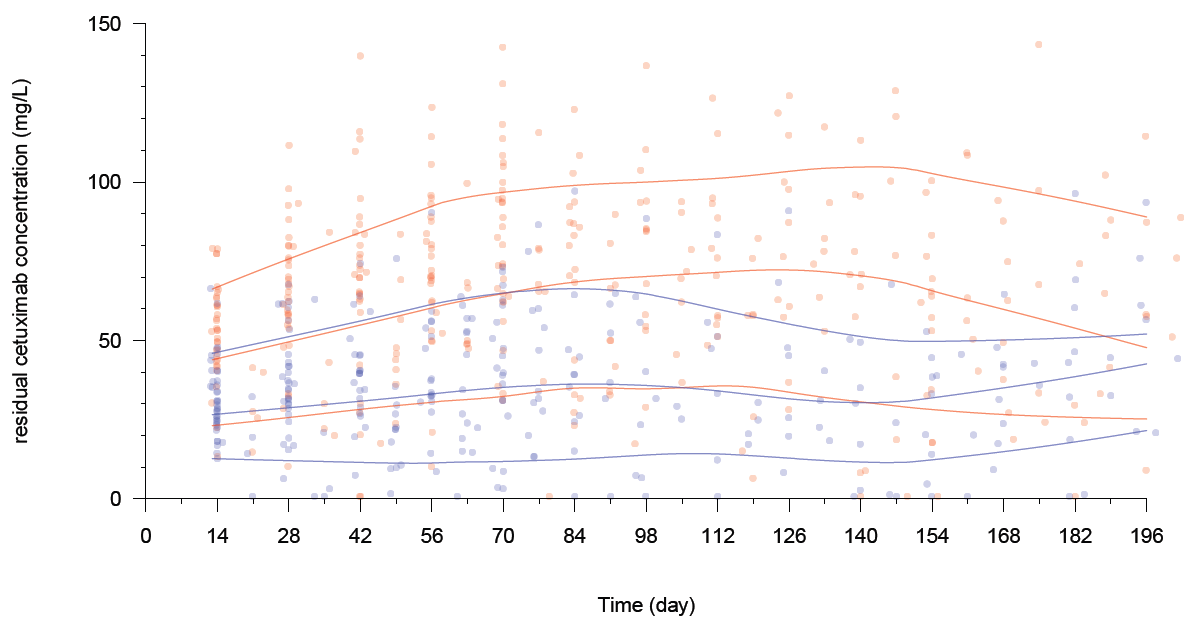
\includegraphics[width=6cm]{figures/raster/FIG_29}
	\caption{Concentrations résiduelles au cours du temps, en fonction de la clairance globale. En bleu, clairance globale supérieure à la valeur médiane ; En rouge, clairance globale inférieure. Les lignes correspondent aux 5éme, 50éme et 95éme percentiles dans les deux groupes.}
	\label{fig:29}
\end{figure}
Dans notre étude, les concentrations résiduelles les plus nombreuses étaient celles de J14 (avant la troisième injection de cetuximab, $n = 71$) et J28 (avant la cinquième injection, $n = 62$). Après avoir contrôlé la corrélation entre ces concentrations et les valeurs de clairance globale (Figure~\ref{fig:33}), nous avons quantifié leur relation  avec la PFS. Les patients dont la concentration résiduelle à J14 était supérieure à la valeur médiane avaient un risque relatif de progression 1,9 fois plus faible que les autres patients ($p = 0,014$). Les patients dont la concentration résiduelle à J28 était supérieure à la valeur médiane avaient un risque relatif de progression également 1,9 fois plus faible que les autres patients ($p = 0,025$) (Figure~\ref{fig:31}).
\begin{figure}[htbp]
	\centering
		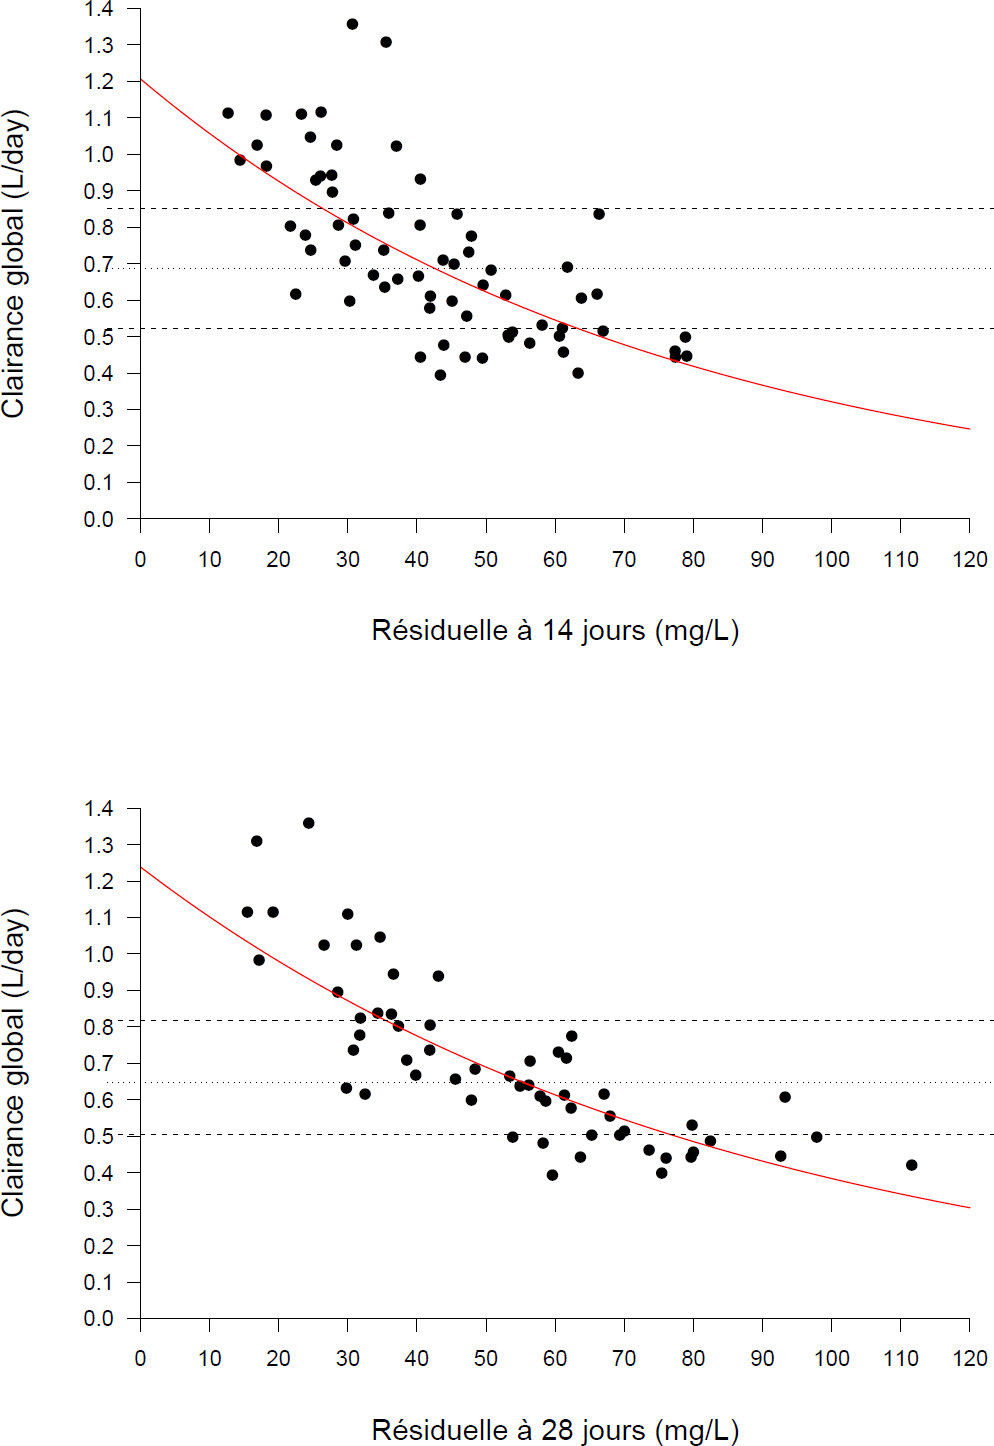
\includegraphics[width=6cm]{figures/raster/FIG_30}
	\caption{Clairances globales des patients représentées en fonction des concentrations résiduelles à J14 (en haut) et à J28 (en bas). Les courbes représentent des régressions exponentielles, les droites en pointillés représentent le 25éme, 50éme et 75éme percentile des clairances globales.}
	\label{fig:30}
\end{figure}
\begin{figure}[htbp]
	\centering
		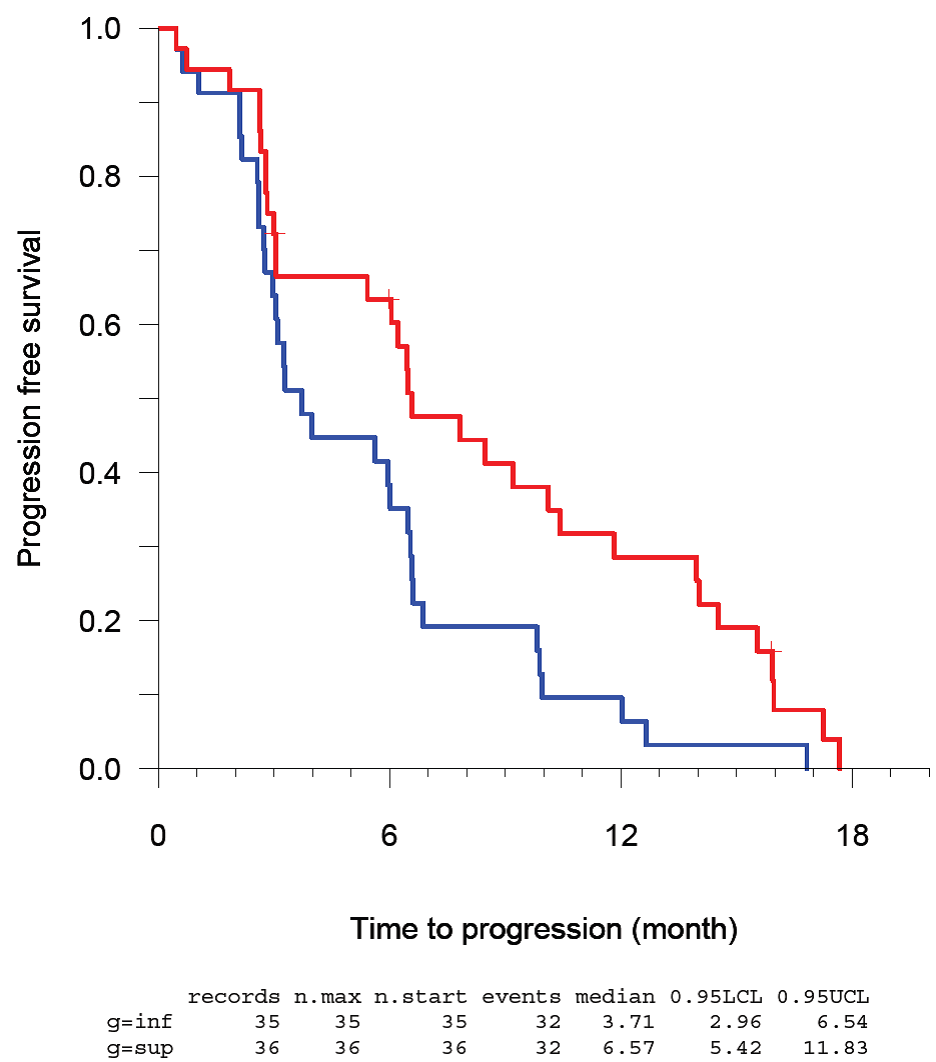
\includegraphics[width=6cm]{figures/raster/FIG_31a}
		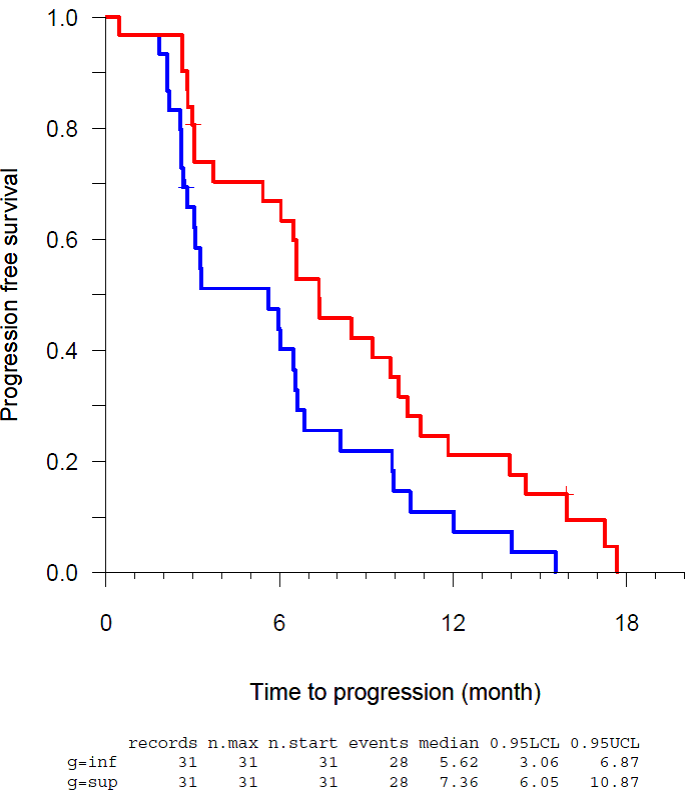
\includegraphics[width=6cm]{figures/raster/FIG_31b}
	\caption{Survie sans progression (PFS) selon la concentration résiduelle de cetuximab avant réinjection. A gauche, concentration résiduelle à J14 ($p = 0,014$) ; a droite, concentration résiduelle à J28 ($p = 0,025$) - En rouge, patients ayant une concentration résiduelle supérieure ou égale à la médiane ; en bleu, patients ayant une concentration résiduelle inférieure à la médiane.}
	\label{fig:31}
\end{figure}
\subsection{Conclusion}
Cette étude a permis de montrer l'influence de l'exposition au cetuximab sur la survie sans progression de patients traités pour cancer colorectal métastatique. Le statut \textit{KRAS} des tumeurs n'était pas directement associé à la survie sans progression. Les deux principales hypothèses pour expliquer cette absence d'influence sont celle d'un manque de puissance statistique due à un faible nombre de patients et celle d'une compensation du manque d'effet du cetuximab chez les porteurs de tumeurs mutées \textit{KRAS} par la chimiothérapie individualisée associée. Le statut \textit{KRAS} a initialement été identifié comme influençant significativement la PFS, sur un nombre moins important de patients~\citep{REF110}. La première hypothèse optant pour un manque de puissance statistique est donc peu plausible. La seconde hypothèse est en revanche plus intéressante. Pour la confirmer, il sera nécessaire de quantifier l'effet des trois médicaments dans un même modèle. Cependant, pour des raisons éthiques, le cetuximab n'est maintenant plus administré aux patients porteurs de tumeurs \textit{KRAS} mutées. Les données de l'étude FOLFIRICETUX sont donc parmi les dernières permettant de quantifier une éventuelle compensation de l'effet des médicaments entre eux. Il serait donc intéressant d'analyser l'influence des concentrations de 5-FU et d'irinotecan sur la relation concentration-effet du cetuximab.

Par ailleurs, le cetuximab a été arrêté relativement tôt chez les six patients \textit{FCGR3A}-V/V, ce qui pourrait expliquer l'absence d'influence significative de ce génotype sur la PFS de nos patients. 

Enfin, nous avons pu mettre en évidence à la fois une relation entre la clairance globale du cetuximab et la concentration sérique résiduelle à J14, et une relation entre cette concentration et la PFS. Ce résultat pourrait permettre d'adapter individuellement la posologie de cetuximab rapidement après l'initiation du traitement si l'intérêt d'une telle procédure est confirmé de façon prospective.

\section{Simulation des concentrations obtenues avec différentes posologies de cetuximab (manuscrit IV)}
\subsection{Contexte}
Dans le cadre du traitement du cancer colorectal métastatique et du cancer ORL, le cetuximab est approuvé pour être administré avec une dose de charge de 400~mg/m$^2$ suivi de perfusions de $250 mg/m^2$ toute les semaines. Cette posologie a montré son efficacité, mais l'intervalle d'injection ($\tau$) n'est pas adapté à celui d'une chimiothérapie concomitante. En effet, pour le cancer colorectal, les injections d'irinotecan ou de 5-fluorouracile (5-FU) sont espacées de deux semaines. Pour le confort du patient, l'injection d'une double dose de cetuximab ($500 mg/m^2$) toute les deux semaines est une posologie de plus en plus utilisée. Cependant, les études visant à justifier l'équivalence de cette posologie avec celle recommandée ne se basent que sur la comparaison des toxicités cutanées ou des réponses cliniques dans des petites cohortes~\citep{REF118}, ~\citep{REF136, REF137, REF138}. Dans le traitement du cancer ORL, la chimiothérapie est administrée toute les trois semaines~\citep{REF105, REF106}. Il est donc également envisagé d'ajuster l'intervalle d'injection du cetuximab à celui de la chimiothérapie dans cette pathologie. 

La variabilité de la pharmacocinétique du cetuximab a été rapportée dans différentes études~\citep{REF68, REF122} ainsi que dans les études des publications~II et III. Une relation entre les concentrations résiduelles de cetuximab et la réponse objective a été décrite précédemment~\citep{REF122}. Cette étude montre que les patients en progression ont des concentrations résiduelles moyennes autour de 30 mg/L alors que les patients stables ou répondeurs ont des concentrations résiduelles moyennes autour de 60 mg/L~\citep{REF122}. Dans la publication III, nous avons également montré que la clairance globale du cetuximab ainsi que la concentration résiduelle à 14 jours, qui en est le reflet, étaient des facteurs reliés significativement avec la survie sans progression (PFS). Il est également reconnu que la pharmacocinétique du cetuximab est dose-dépendante, car elle fait intervenir une élimination saturable~\citep{REF68, REF118, REF123, REF127, REF128}. Cette dose-dépendance rend le choix de posologies équivalentes complexe et peut entraîner une sous-exposition des patients recevant du cetuximab toute les deux ou trois semaines si la posologie est fondée sur une pharmacocinétique considérée comme linéaire.

L'étude de l'équivalence entre différentes posologies de cetuximab doit comparer l'efficacité des traitements, mais doit tout d'abord être fondée sur une bonne description de l'exposition des patients. Nous avons utilisé les paramètres de population obtenus lors de l'analyse de la pharmacocinétique du cetuximab chez des patients traités pour cancer colorectal métastatique (publication~III) pour simuler l'exposition de patients virtuels traités par cetuximab avec différentes posologie, faisant intervenir différentes doses injectées toutes les une, deux ou trois semaines.
\subsection{Simulations}
A l'aide d'une cohorte virtuelle de 1000 patients générés avec les valeurs des paramètres pharmacocinétiques du modèle de la publication~III, nous avons simulé 3 essais cliniques, avec les trois posologies de cetuximab suivantes :
\begin{description}
\item[Posologie~1 :] Dose de charge de 400~mg/m$^2$ suivie de 250~mg/m$^2$ toute les semaines (posologie approuvée).
\item[Posologie~2 :] Dose de 500~mg/m$^2$ de cetuximab toute les deux semaines (posologie déjà utilisée en clinique).
\item[Posologie~3 :] Dose de 750~mg/m$^2$ de cetuximab toute les trois semaines (correspondant à 3$\times$250~mg/m$^2$ toute les semaines)
\end{description}

\subsection{Analyses}
Les trois différents profils pharmacocinétiques obtenus avec les différentes posologies présentaient des différences importantes en termes de concentrations résiduelles (Figure~\ref{fig:32}). La posologie~3 entrainait les concentrations résiduelles de cetuximab les plus faibles, avec une médiane à 48~mg/L et plus de 5\% des patients en deçà de 30~mg/L. Les quantiles des distributions des concentrations résiduelles sont présentés dans le tableau~\ref{tab:4} suivant. 



\begin{table}[htbp]
\caption{Quantiles des distributions des concentrations résiduelles et des $AUC$ cumulées de cetuximab à 84~jours en fonction de la posologie, pour 1000~patients virtuels}
\scriptsize
%\begin{tabularx}{\textwidth}{XX|m{.05\textwidth}m{.05\textwidth}m{.06\textwidth}m{.05\textwidth}m{.05\textwidth}|m{.05\textwidth}m{.05\textwidth}m{.06\textwidth}m{.05\textwidth}m{.05\textwidth}|}
%\begin{tabularx}{\textwidth}{p{2em}p{2em}|XXXXX|XXXXp{2em}|}
%\multicolumn{2}{p{4em}}{\,}	&\multicolumn{5}{|m{.3\textwidth}}{Quantiles des concentrations résiduelles de cetuximab à 84 jours (mg/L)}	
%& \multicolumn{5}{|m{.4\textwidth}|}{Quantiles des $AUC$ cumulées de cetuximab à 84 jours (g/L/jour)} 	\\
%\hline
%\hline
%      Doses (mg/m$^2$) & $\tau$ (semaine) & Mini & 5\% & médiane & 95\% & Maxi & Mini & 5\% & médiane & 95\% & Maxi \\
%      400 - 250 & 1 & 44,6 & 63,1 & 84,3 & 111,9 & 137,6 & 7,8 & 8,9 & 10,4 & 12,4 & 13,8 \\
%      500 & 2 & 30,5 & 42,9 & 63,0 & 88,7 & 115,9 & 7,5 & 8,7 & 10,1 & 12,1 & 13,5 \\
%      750 & 3 & 17,3 & 29,2 & 48,0 & 72,1 & 99,3 & 7,7 & 8,9 & 10,4 & 12,4 & 13,9 \\
%      \hline
%    \end{tabularx}
  \label{tab:4}
\end{table}


\subsection{Conclusions}
Nos résultats objectivent les conséquences potentielles de la non-linéarité du cetuximab sur ses concentrations sériques lors de l'espacement des injections. Bien que les différences observées en termes d'$\AUC$ ne soient pas cliniquement pertinentes, les différences en termes de concentrations résiduelles à l'équilibre sont importantes et leur pertinence doit être étudiée. De plus, l'espacement des injections associé à une augmentation proportionnelle de la dose des perfusions entraine de grands écarts entre les concentrations avant et après injection (pic). Nos résultats donnent des outils pour une adaptation posologique raisonnée lors de l'augmentation des intervalles de perfusion. Nos résultats doivent bien entendu être confirmés par des études pharmacocinétiques prospectives.
\begin{figure}[htbp]
	\centering
		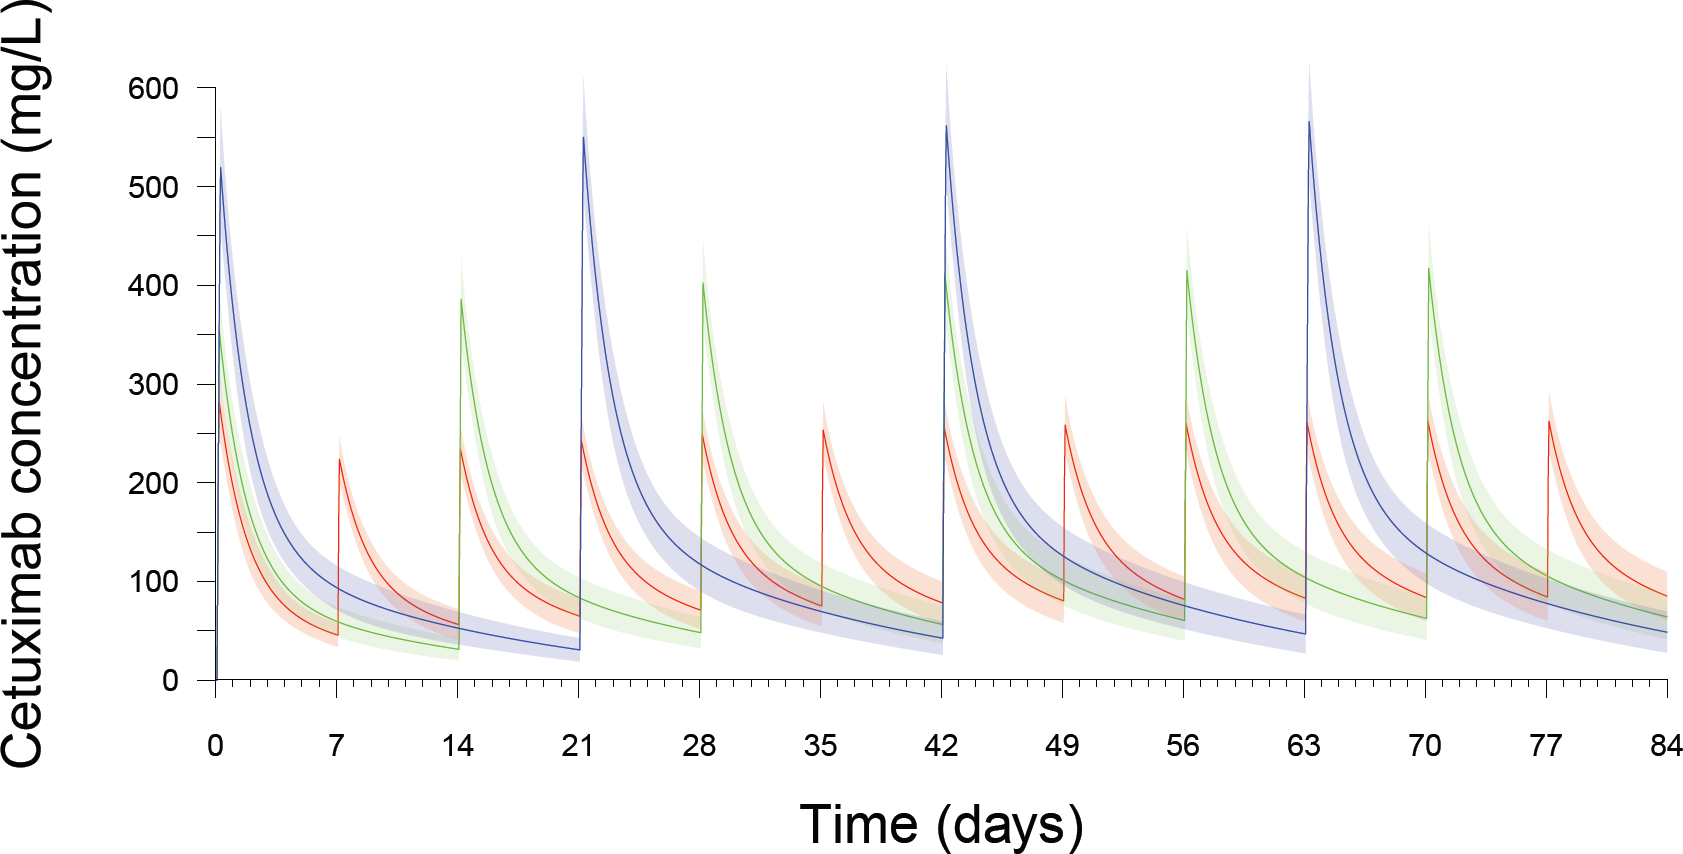
\includegraphics[width=10cm]{figures/raster/FIG_32a}
		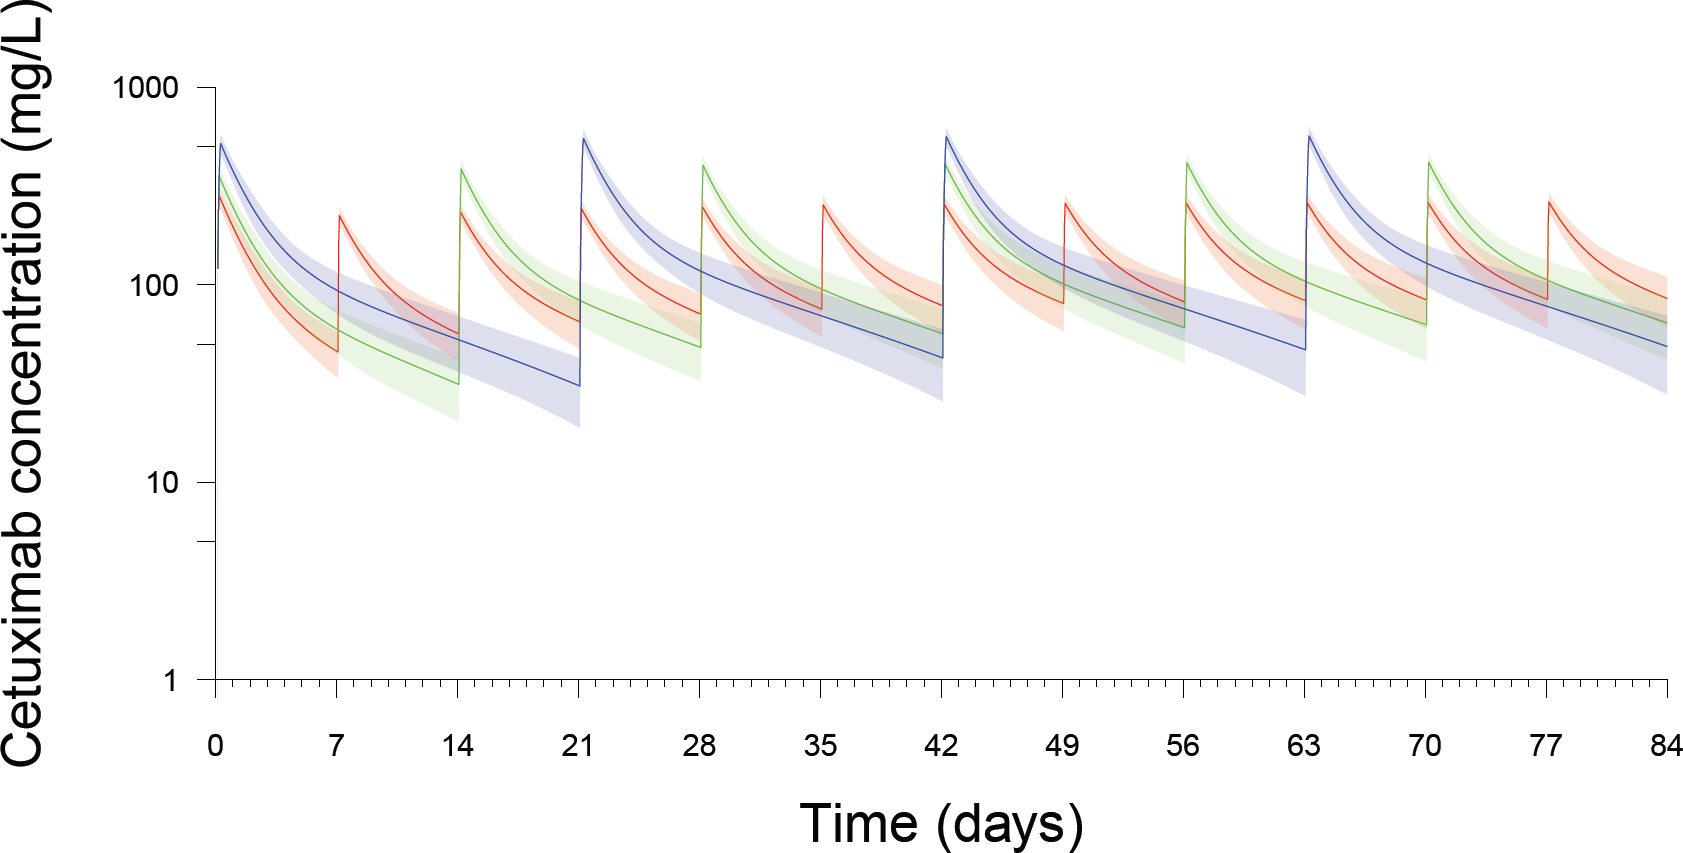
\includegraphics[width=10cm]{figures/raster/FIG_32b}
	\caption{Concentrations de cetuximab simulées avec trois différentes posologies ayant la même dose cumulée sur trois semaines.(Médiane et 90\% \textbf{interval of the patients}) – En rouge, 400~mg/m$^2$ suivie de 250~mg/m$^2$ toute les semaines – En vert, 500~mg/m$^2$ toute les deux semaines – En bleu, 750~mg/m$^2$ toute les trois semaines.}
	\label{fig:32}
\end{figure}
\section{Étude de l'absorption pulmonaire du cetuximab dans un modèle murin (publication~V)}
\subsection{Contexte}
Un des problèmes majeurs associé à l'utilisation du cetuximab est sa toxicité, notamment cutanée, qui limite parfois son emploi 139. Dans le cas du cancer broncho-pulmonaire, son administration par voie inhalée pourrait permettre d'augmenter sa concentration au niveau du site tumoral dans le poumon tout en diminuant sa toxicité systémique. En effet, la présence de FcRn dans le poumon a été montrée~\citep{REF27} et les travaux de Maillet \textit{et al}. ont démontré in vitro la possibilité de nébuliser le cetuximab tout en conservant ses propriétés de fixation à l'EGFR~\citep{REF140}. L'objectif de l'étude était d'analyser par modélisation pharmacocinétique la biodisponibilité du cetuximab administré par nébulisation chez la Souris. L'analyse de ce modèle préclinique était en effet indispensable dans le cadre du développement de cette potentielle nouvelle voie d'administration. Afin de décrire l'évolution des concentrations au cours du temps et d'analyser la biodisponibilité du cetuximab, une modélisation pharmacocinétique a été réalisée à la fois par approches non-compartimentale et compartimentale. 

\subsection{Modèle murin}
Des cellules A431 issues de lignées cellulaires de carcinome épidermoïde cutané ont été obtenues auprès de l'ATCC (American Type Culture Collection). Ces cellules surexpriment de manière constitutive l'EGFR et représentent les cellules de référence pour les études du cetuximab~\citep{REF141}. Dans cette étude, 2,5 $\times 10^6$ cellules ont été instillées par voie endotrachéale chez 13 souris (femelles nude Balb/c de 5 semaines). Le dépôt des cellules marquées par du 99mTc a été suivi par scintigraphie. Six à sept semaines plus tard, les souris ayant développé une tumeur de taille supérieure à 1 mm ont reçu 60 à 80 $\mu$g de cetuximab-Xenofluor750 par voie IV (groupe~IV, $n = 7$) ou par nébulisation dans l'arbre respiratoire (groupe nébulisation, n = 6). Des échantillonnages de sang de 100 à 200 $\mu$L, à H0, H2, H8, J1, J3, J7 et J14 ont permis de mesurer les concentrations sériques de cetuximab par méthode ELISA.
\subsection{Modélisation de la pharmacocinétique}
En ce qui concerne l'approche non-compartimentale, l'$\AUC$ de chaque souris a été estimée par la méthode des trapèzes (équations~\ref{eq:2}~et~\ref{eq:3}). Les moyennes étaient respectivement de 612 et 55,2 h$\times \mu$g/L pour les souris du groupe~IV et nébulisation. La fraction d'$\AUC$ extrapolée n'excédait pas 2,5\% sauf pour une souris du groupe nébulisation (27,15\%). La fraction biodisponible $F$ (équation~\ref{eq:5}), estimée à partir des deux groupes parallèles de souris, était de 9\%. Les moyennes (équations~\ref{eq:7}~et~\ref{eq:8}) étaient respectivement de 59185 et 6745,5 h$^2\dot \mu g/L$ pour les souris du groupe~IV et nébulisation. Le temps de résidence moyen $MRT$ (équation~\ref{eq:6}) était en moyenne de 95 h pour le groupe~IV et de 111,5 h pour le groupe nébulisation. Le temps d'absorption moyen MAT était donc de 34 h. 

L'approche compartimentale a d'abord été réalisée en séparant les groupes. Cependant, la vitesse d'absorption ne permettant pas de bien identifier les paramètres de distribution après nébulisation, les deux voies d'administration ont été analysées de façon conjointe. Le modèle utilisé était bicompartimental avec un compartiment d'absorption pour les souris du groupe nébulisation (équation 19). Les valeurs initiales des paramètres ka et F ont été obtenues par les équations 23 et 5 grâce aux résultats de l'analyse non-compartimentale. Ce modèle a permis une description satisfaisante des concentrations. Les estimations des paramètres et leurs CV interindividuels était $V_1$ = 5,73~mL (6,3\%), $\CL$ = 0,12~mL$\cdot$h$^{-1}$ (13\%) $V_2$ = 9,16~mL (9,6\%), $Q$ = 0,63~mL$\cdot$h$^{-1}$ (16\%) et pour le groupe nébulisation, $k_a$ = 0,04~h$^{-1}$ (25\%). Le poids des souris n'influençait pas significativement les paramètres du modèle.
\begin{figure}[htbp]
	\centering
		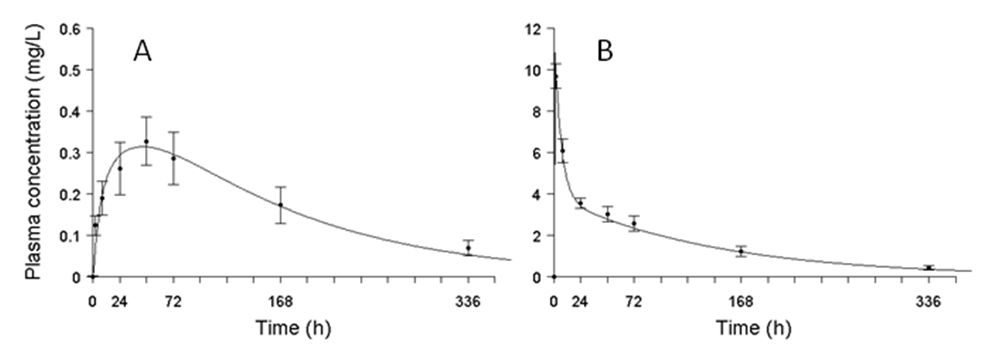
\includegraphics[width=10cm]{figures/raster/FIG_33}
	\caption{Pharmacocinétique du cetuximab chez la Souris, administré par voie nébulisée (A) et par voie IV (B). Les points représentent les concentrations moyennes ainsi que les écart-types observées pour les souris de chaque groupe. Les traits représentent les concentrations prédites par le modèle final. A noter : l'échelle des concentrations est différente selon la voie d'administration.}
	\label{fig:33}
\end{figure}

\subsection{Conclusions}
La comparaison des profils pharmacocinétiques après administration de cetuximab par nébulisation (Figure~\ref{fig:33}A) et IV (Figure~\ref{fig:33}B) chez la Souris a permis de décrire la phase d'absorption en quantifiant une constante d'absorption $k_a$ et une fraction absorbée $F$. La bonne description de cette absorption par une constante d'ordre~1 suggère que le FcRn pulmonaire, qui est vraisemblablement le principal acteur du passage des IgG à travers la barrière alvéolo-capillaire~\citep{REF27}, n'est pas saturé chez la Souris aux doses utilisées.

Dans le cas d'un cancer broncho-pulmonaire, l'effet recherché du cetuximab est locorégional. La faible fraction absorbée ($F$ = 9 à 11\%) et la persistance du cetuximab dans le poumon ($MAT$ de 34 h et persistance du marquage pulmonaire par le Xenofluor) suggèrent une bonne exposition des tissus pathologiques après nébulisation. Dans le modèle murin utilisé, l'administration de cetuximab en aérosol a permis une régression significative de la masse tumorale (Publication V, Figure 5A).
